%                                                                 aa.dem
% AA vers. 8.3, LaTeX class for Astronomy & Astrophysics
% demonstration file
%                                                       (c) EDP Sciences
%-----------------------------------------------------------------------

\documentclass{aa}  
%\documentclass[referee]{aa}        % for a referee version
%\documentclass[onecolumn]{aa}      % for a paper on 1 column  
%\documentclass[longauth]{aa}       % for the long lists of affiliations 
%\documentclass[rnote]{aa}          % for the research notes
%\documentclass[letter]{aa}         % for the letters 
%\documentclass[bibyear]{aa}        % if the references are not structured 
                                    % according to the author-year
                                    % natbib style

%%%%%%%%%%%%%%%%%%%%%%%%%%%%%%%%%%%%%%%%
\usepackage{natbib}
\usepackage{graphicx}
\usepackage{txfonts}
\usepackage{hyperref}
\usepackage{color}
%%%%%%%%%%%%%%%%%%%%%%%%%%%%%%%%%%%%%%%%
% To add links in your PDF file, use the package "hyperref"
% with options according to your LaTeX or PDFLaTeX drivers.
\usepackage{url,twoopt,amssymb}

% define link colors
\hypersetup{
  colorlinks=true,   %% links colored instead of frames
  urlcolor=blue,     %% external hyperlinks
  linkcolor=blue     %% internal latex links (eg Fig)
}


\begin{document}
  \title{On the stability of the ICRF axes}
%   \subtitle{I. Overviewing the $\kappa$-mechanism}
  \author{N. Liu\inst{1,2}
     \and
          S. B. Lambert\inst{3} %\fnmsep
          \and
          F. Arias\inst{3}
          \and
          J.-C. Liu\inst{1}
          \and
          Z. Zhu\inst{1}
          }

  \institute{School of Astronomy and Space Science,
   		     Key Laboratory of Modern Astronomy and Astrophysics (Ministry of Education), Nanjing University, Nanjing 210023, P. R. China\\
              \email{[niu.liu;jcliu;zhuzi]@nju.edu.cn}
         \and
             School of Earth Sciences and Engineering, Nanjing University, Nanjing 210023, P. R. China
         \and
             SYRTE, Observatoire de Paris,
             Universit\'e PSL, CNRS, Sorbonne Universit\'e, LNE, Paris, France\\
             \email{sebastien.lambert@obspm.fr}
             }

  \date{Received; accepted}


  \abstract
  % context heading (optional)
  % {} leave it empty if necessary
   {
   }
  % aims heading (mandatory)
   {
   }
  % methods heading (mandatory)
   {
   }
  % conclusions heading (optional), leave it empty if necessary 
   {}

  \keywords{reference systems -- 
            astrometry --
            techniques: interferometric --
            quasars: general --
            catalogs}

\maketitle

%________________________________________________________________

\section{Introduction}

    The celestial reference frame (CRF) provides the basic position reference widely used in the astronomy and geoscience.
    The current realization of the CRF as adopted by the International Astronomical Union (IAU) in 2018 is the third realization of the International Celestial Reference Frame \cite[ICRF3;][]{2020A&A...644A.159C}.
    The ICRF3 is materialized by positions of more than 4000 extragalactic sources based on very long baseline interferometry (VLBI) observations made at the dual $S/X$-, $K$-, and $X/Ka$-band since 1979.
    With several improvements in the modelling, for example, the correction of the Galactic aberration effect due to the acceleration of the solar system barycenter \citep{2019A&A...630A..93M}, and more accumulated data, the best position precision achieved for individual sources in the ICRF3 has reach a level of 30 micro-arcsecond ($\mathrm{\mu as}$).
    
    The extragalatic sources are used to construct the ICRF because they are distant from us so that they appear more compact than other objects like Galatic stars with a stable position in the sky.
    However, the apparent position of the extragalatic source varies with time, both in the radio and optical domain \cite[e.g., see][]{2009jsrs.conf..199A,2013A&A...553A.122L}.
    This kind of position variability of extragalatic sources, sometimes also referred to as the astrometric stability, would lead to variations in the direction of the celestial frame axes defined by positions of those sources.
    This phenomenon is known as the celestial frame instability \cite[e.g.,][]{2008A&A...481..535L}, a common issue for all kinds of extragalatic celestial reference frame such as the ICRF and the \textit{Gaia} celestial frame \cite[\textit{Gaia}-CRF;][]{2018A&A...616A..14G}.
    This celestial frame instability would introduce additional noises to the VLBI products such as the Earth orientation parameters (EOP); the implication would be more serious for the nutation series since so far the VLBI is the sole technique that can determine the nutation angle.
    \citet{2003JGRB..108.2275D,2008A&A...481..535L} study the impact of the celestial frame instability on the estimate of the nutation terms from the VLBI observations and report an additional noise of $\mathrm{15\,\mu as}$ in the amplitude of 18.6-year nutation term.
    The variability of extragalatic source might also degrade the precision of VLBI-\textit{Gaia} frame link \citep{2013A&A...552A..98T,2016A&A...587A.112T,2018A&A...611A..52T}.
    Therefore, it is necessary to assess and monitor the instability level of the celestial reference system.
    This work focuses on the axis stability of the ICRF materialized by VLBI observations.
    
    There are several possibilities that make radio source apparent position unstable.
    The main origin is the temporal evolution of radio source structure due to intrinsic variability such as the ejection of new jet features, which could manifest itself as an apparent proper motion (linear drift) of radio sources \citep{2011AJ....141...91F,2011AJ....141..178M}.
    Other causes include the difference of radio source position as ``seen'' by different VLBI network \citep{2003JGRB..108.2275D} and the weak micro-lensing effect \citep{1998MNRAS.300..287S}.    
    
    Several authors have proposed indicators to characterize the radio source position stability.
    Statistics based on the source coordinate time series are often used, e.g., slope and standard deviation \citep{2003A&A...403..105F}, Allan variance \citep{2018A&A...618A..80G}.
    The ICRF Working Group uses a quantity considering the coordinate variations (weighted root-mean-square, WRMS) and the reduced chi-square for right ascension and declination \citep{2015AJ....150...58F,2020A&A...644A.159C}.
    In addition, other authors construct indicators based on the interstellar scintillation around the source \citep{2013MNRAS.434..585S} and flux density time series \citep[light curve;][]{2014JGeod..88..575S}, which are found to be correlated with the position stability.
    Based on these indicators, sources with an unstable positions can be recognized and ruled out, leaving these stable sources to define and maintain the axes of the ICRF, which is known as the so-called defining source \citep{2003A&A...403..105F,2006A&A...452.1107F,2009A&A...493..317L}.
    The stability of the VLBI celestial reference frame can be thus improved when a proper ensemble of stable sources are used as the defining source \citep{2004A&A...422.1105A,2017MNRAS.466.1567L}.
    
    The ICRF axes are found to be stable on a level of $\mathrm{20\,\mu as}$ \citep{1998AJ....116..516M}, which is further improved to $\mathrm{10\,\mu as}$ for the ICRF2 \citep{2015AJ....150...58F}.
    These results are based on comparing the relative orientation of various subsets of sources.
    Adopting a different method, \citet{2013A&A...553A.122L} constructs the yearly celestial reference frame from the radio source coordinate time series.
    The author finds that the axis stability of the ICRF2 does not degrade after 2009, which is around $\mathrm{20\,\mu as}$ for each axis.
    Later, \citet{2014A&A...570A.108L} compares VLBI radio source catalogs submitted from different analysis centers of the International VLBI Service for Geodesy and Astrometry \citep[IVS;][]{2017JGeod..91..711N} and reports an agreement of several tens of $\mathrm{\mu as}$ among these catalogs.
    Recently, \cite{2018A&A...618A..80G} study the astrometric stability of extragalactic sources in the light of the Allan standard deviation of VLBI position time series.
    They conclude that the source position showing a stable behavior is likely to become unstable within a longer time span.
    It highlights the need of regularly monitoring the astrometric behaviors of radio sources and the axis stability of the ICRF, as already pointed out in \citet{2013A&A...553A.122L}.
    
    This work aims to re-assess the stability of ICRF axes.
    To achieve this goal, we adopted different methods used in the literature as well as developed our own method (Sect.~\ref{sec:methods}) and compared the results (Sect.~\ref{sec:results}).
    Considering that the ICRF3 is materialized in three frequencies and that the \textit{Gaia} catalog also provide an optical realization of the ICRF, we evaluated the agreement of the axis direction of these catalogs (Sect.~\ref{subsec:axis-agreement}).
    This analysis serves as a check of the consistency of ICRF axes at different frequencies and also a preview of the potential precision of the VLBI-\textit{Gaia} frame link.


%__________________________________________________________________

\section{Data}  \label{sec:data}

%______________________________________________________________

\subsection{Catalogs}  \label{subsec:catalogs}

%__________________________________________________ One column table
\begin{table}
    \centering
    \caption[]{Statistics of number of sources in catalogs used in this work.}
    \label{tab:cat-stats}
    \begin{tabular}{ccccc}
        \hline
        \noalign{\smallskip}
        Catalog     &All    &Com. to        &ICRF3   \\
                    &       &ICRF3 $S/X$    & Def.   \\
        \noalign{\smallskip}
        \hline
        \noalign{\smallskip}
        ICRF2           &3414   &3410   &296 \\ 
        ICRF3 $K$       & 793   & 550   &193 \\
        ICRF3 $X/Ka$    & 638   & 450   &176 \\
        asi2020a        &4447   &4296   &290 \\
        aus2020b        &4817   &4456   &299 \\
        opa2021a        &5517   &4490   &303 \\
        usn2019c        &2390   &2263   &292 \\
        \noalign{\smallskip}
        \hline
    \end{tabular}
\end{table}
    
    The ICRF3 catalog \citep{2020A&A...644A.159C} was retrieved from the Paris Observatory IERS ICRS center. \footnote{\url{https://hpiers.obspm.fr/icrs-pc/newwww/icrf/index.php}}
    We took the AGN sample (\texttt{gaiaedr3.agn\_cross\_id} table) in the \textit{Gaia} EDR3 from the \textit{Gaia} archive\footnote{\url{http://gea.esac.esa.int/archive/}}, where we found optical counterparts for 3181 ICRF3 sources via the external catalog name (column ``\texttt{catalogue\_name}'') for identifying these sources.
    There are 3142 sources in the \textit{Gaia} EDR3 common to the ICRF3 $S/X$-band catalog, 660 common to the $K$-band catalog, and 576 for the $X/Ka$-band.
    % This subset is denoted as the \textit{Gaia}-CRF3 solution in the content.
    
    We used four radio source catalogs which are publicly available at the IVS data center.\footnote{These catalogs are available via anonymous ftp to \url{ftp://ivsopar.obspm.fr/vlbi/ivsproducts/crf}. The technical description of these solutions can be found at \url{ftp://ivsopar.obspm.fr/vlbi/ivsdocuments/}.}
    These solutions were: asi2020a from the the Space Geodesy Centre of the Italian Space Agency, aus2020b from the Geoscience Australia, opa2021a from the Paris Observatory, and usn2019c from the Unites States Naval Observatory.
    The solution aus2020b was obtained with the OCCAM geodetic VLBI analysis software package \citep{2004ivsg.conf..267T}, while the rest catalogs were obtained from the Calc/Solve package developed and maintained by the VLBI group at NASA/GSFC \citep{1986AJ.....92.1020M}.
    Sources whose position was estimated with no more than three observables were removed from the list; this was done for all four catalogs.
    
    Table~\ref{tab:cat-stats} tabulates statistics of number of sources in these catalogs mentioned above, as well as the subset of sources common among them.

%______________________________________________________________

\subsection{VLBI observations and global solutions}  \label{subsec:vlbi-data}

    We used the dual $S/X$-band VLBI observations made during 1979-2021, in total 6864 regular sessions and nearly 15 million observables (group delays). \footnote{A regular session is a collection of VLBI observations made within 24 hours (a day). The full session list can be found at \url{http://ivsopar.obspm.fr/24h/opa2021a.arc}, whereas sessions after January 1st, 2021 therein were used in this work.}
    These data were reprocessed by the Calc/Solve in the global solution mode, following an identical setup and parameterization to the solution opa2021a.
    The detailed technique description can be found at the Paris Observatory Geodetic VLBI Center. \footnote{\url{http://ivsopar.obspm.fr/24h/opa2021a.eops.txt}}
    In the resulting radio source catalogs, sources whose position was estimated with less than three group delays were also removed.

%______________________________________________________________

\subsection{Radio source coordinate time series}  \label{subsec:ts-data}

%   We used the radio source coordinate time series available at Paris Observatory Geodetic VLBI Center.\footnote{\url{http://ivsopar.obspm.fr/radiosources/index.php}}
%   These time series are derived from the geodetic/astrometric VLBI observations starting from 1979 and will be periodically updated.
%   The parameterization and a priori model choice of the VLBI solutions were almost identical to those used for deriving the opa2021a solutions, except some special configurations of radio source position and celestial frame maintenance; for later we referred to \citet{2013A&A...553A.122L} for a detailed description.
%   We downloaded the coordinate time series for 4879 radio sources on on March 15, 2021, which were derived based the VLBI observations spanning from 1979.6 to 2021.2.
%   There are 4538 sources in common with the ICRF3 catalogs, including all the 303 ICRF3 defining sources.
%   These data will be used to derive the apparent proper motion of the radio source and construct yearly celestial reference frame.
    \textbf{The radio source coordinate time series were derived through several \textcolor{red}{(actual number?)} separate global solutions, following the same setup and parameterization of the opa2021a solution except some special configurations of radio source position estimate and celestial frame maintenance; for later please refer to \citet{2013A&A...553A.122L} for a detailed description.
    The coordinate time series were obtained for 4827 sources, including all the 303 ICRF3 defining sources.
   These data will be used to derive the apparent proper motion of the radio source and construct yearly celestial reference frame.}

   
%______________________________________________________________

\section{Methods}  \label{sec:methods}

    The axis stability of the celestial frames were evaluated by three methods:
   \begin{enumerate}
      \item We estimated the apparent proper motions (slope) from coordinate time series of extragalactic sources and then fitted the global spin vector based on these apparent proper motions.
      The spin multiplied by the time span gives an estimate of the axis stability.
    %   \citet{}
      \item We constructed the yearly celestial reference frame from the coordinate time series and VLBI global solutions of observations with different time span, respectively, and compared the  relative orientation of these yearly CRFs with referred to the ICRF3 $S/X$-band catalog.
      The dispersion of the relative orientation angles provides a metrics of the stable stability.
      \item We compared various representations of the ICRF from VLBI global solutions with different analysis strategies and fitted the relative orientation of these representations with referred to the ICRF3 based on the subset of the ICRF3 defining sources.
   \end{enumerate}


%______________________________________________________________

\subsection{Modelling of the global difference}  \label{subsec:vsh}
    
    The global (large-scale) features in any vector filed on the celestial sphere can be described by the vector spherical harmonics (VSH).
    Here we only considered the first degree of the VSH, which consists of a rotation vector \vec{R} and a glide vector \vec{G}.
    The full equation can be expressed as
   %
   \begin{equation} \label{eq:vsh01}
      \begin{array}{ll}
        \Delta_{\alpha^*}  = &-R_1\cos\alpha\sin\delta  - R_2\sin\alpha\sin\delta + R_3\cos\delta \\
                    &-G_1\sin\alpha            + G_2\cos\alpha, \\
        \Delta_{\delta}    = &+R_1\sin\alpha            - R_2\cos\alpha \\
                    &-G_1\cos\alpha\sin\delta  - G_2\sin\alpha\sin\delta + G_3\cos\delta, \\
     \end{array}
   \end{equation}
   %    
   where $\vec{R}=(R_1,R_2,R_3)^{\rm T}$ and $\vec{G}=(G_1,G_2,G_3)^{\rm T}$.
    The rotation vector consists of the rotations around the X-, Y-, and Z-axis and was used to characterize the stability of the ICRF axes.
    
    Since we dealt with the rotation vectors both from the position offset and apparent proper motion vector field, different notations were used for clarity.
    Following the conventions used, e.g., in \citet[][]{2018A&A...616A..14G}, we used the term ``orientation'' to represent the rotation vector estimated from the position offset and ``spin'' for that from the proper motion data, which means that ($\Delta_{\alpha^*}$, $\Delta_{\delta}$) in Eq.~(\ref{eq:vsh01}) were substituted by ($\Delta\alpha^*$, $\Delta\delta$) and ($\mu_{\alpha^*}$, $\mu_\delta$).
    The orientation vector, referred to as $\vec{\epsilon}=(\epsilon_x,\epsilon_y,\epsilon_z)^{\rm T}$, contain three orientation angles of the X-, Y-, and Z-axis among catalogs and can be used to align the catalogs.
    The spin vector $\vec{\omega}=(\omega_x,\omega_y,\omega_z)^{\rm T}$ models the change rate of the ICRF axis direction due to the (apparent) proper motion of extragalatic sources.
    
    The rotation signal was estimated through the least-square (LSQ) fitting to the position offset and proper motion weighted by their formal uncertainties.
    We used an similar algorithm as that in \citet[][]{2020A&A...634A..28L} to remove outliers.
    The rotation and glide vectors are orthogonal to each other, so that the existence of glide (rotation) signal should not affect the estimate of the rotation (glide) parameters for an ensemble of sources uniformly distributing on the sphere.
    However, this condition can never be fulfilled in the real world.
    In this work, the glide parameters were estimated together with the rotation terms in the LSQ fitting in order to reduce possible bias in the estimate of rotation parameters leaked from the glide signal, but will not be discussed or presented.
    We compared the fitted results of the rotation vector with and without including the glide vector in the transformation model and found consistent results within the formal uncertainties.
    
%______________________________________________________________

\subsection{Global rotation signal from bootstrap sampling}  \label{subsec:bs-mathod}
    
    In this work, we mainly estimated the rotation signal using the subset consisted of the ICRF3 defining sources.
    In addition, in order to avoid possible bias when considering exclusively one subset, e.g., unreliable apparent proper motion of some sources, we considered the whole sample and a robust estimate of the global rotation signal was obtained by the bootstrap sampling.
    That is, we picked randomly $N$ sources from the sample (without replacement) and estimated the rotation parameters.
    This procedure was repeated 1000 times and we calculated the mean and standard deviation of the rotation parameters as the estimate value and associated formal uncertainty.
    This method was adopted to estimate the relative orientations between catalogs.
   
%______________________________________________________________

\subsection{Apparent proper motion of radio sources}  \label{subsec:apm-data}

   We estimated the apparent proper motion (linear drift) of the radio source based on their time series through a weighted LSQ fitting.
   This model can be described as following:
   %
   \begin{equation} \label{eq:apm}
      \alpha\cos\delta = \mu_{\alpha*} (t-t_0) + \alpha_0\cos\delta,\ \delta = \mu_\delta (t-t_0) + \delta_0, 
   \end{equation}
   %
   where $\mu_{\alpha*}$ and $\mu_\delta$ are apparent proper motions in the right ascension (R.A.) and declination (decl.), respectively, $t_0$ the mean epoch of the observing span for a given source.
   The notation $\alpha*=\alpha\cos\delta$ will be used throughout this work.
   All the data points were weighted by the inverse of the square of their formal uncertainties.
   Besides, the correlation between the R.A. and decl. were considered in the LSQ fitting, which means that $\mu_{\alpha*}$ and $\mu_\delta$ were fitted simultaneously.
   These data points whose distance to their mean value is greater than three times of their formal uncertainties were removed before estimating $\mu_{\alpha*}$ and $\mu_\delta$ to prevent the possible bias caused by these unreliable measurements.
   Sources with less than five data points in the remaining time series for either R.A. or decl. were also removed from our list.
   We obtained the apparent proper motion for 1484 sources, 290 sources being classified as the so-called ICRF3 defining source.
    
%______________________________________________________________

\subsection{Construction of yearly celestial reference frame}  \label{subsec:yearly-crf}

    Two approaches were used to construct the yearly celestial refe rence frames.
    On the one hand, we truncated the VLBI observations, starting from 1979, at a certain year which ranges from 1985 to 2021 with a step of one year and used these observations as the input of the VLBI global solution.
    Earlier years were not considered due to the scarcity of observations.
    Thus, we ran 37 separated VLBI global solutions.
    On the other hand, we averaged the source position from the coordinate time series within an one-year moving window with a step of also one-year, i.e., without overlaps, since 1985.
    By doing, we formed another version of 36 yearly celestial frames.

%______________________________________________________________

\section{Results}  \label{sec:results}

%______________________________________________________________

\subsection{Global spin from apparent proper motion}  \label{subsec:spin-from-apm}

%______________________________________________ Dist of APM
    \begin{figure}
        \label{fig:apm-dist}%
        \centering
        % 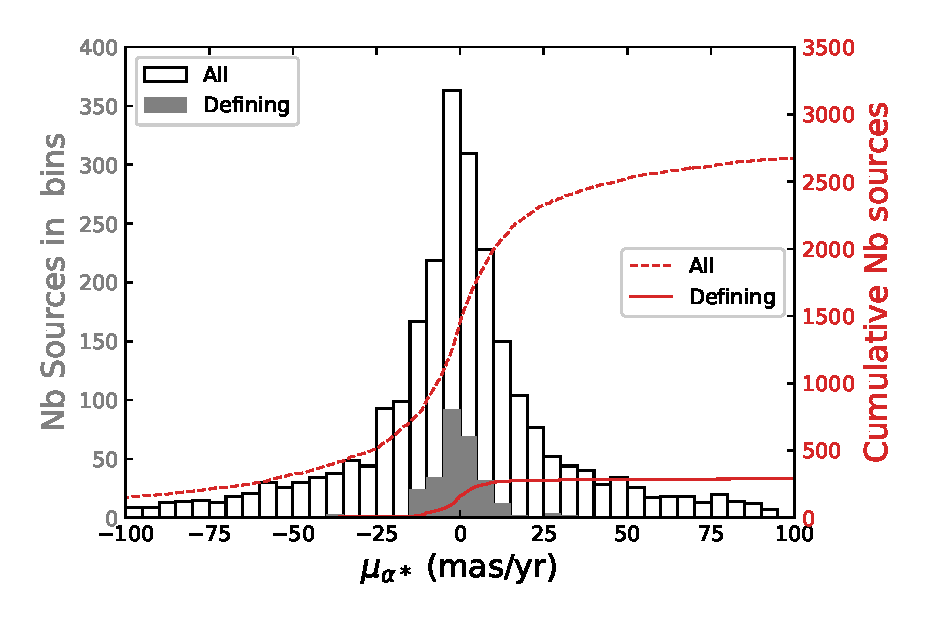
\includegraphics[width=\columnwidth]{figs/pmra-hist}
        % 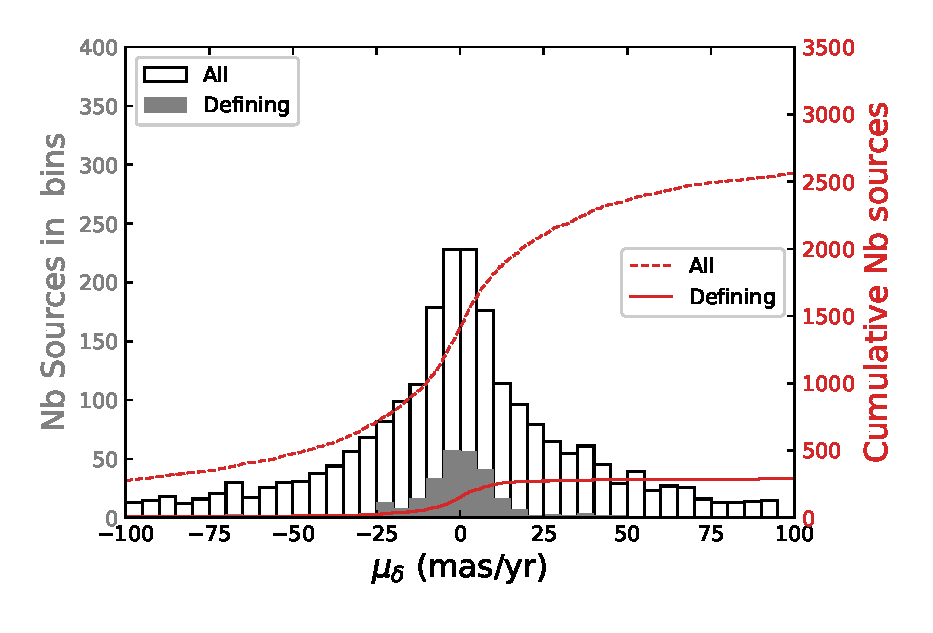
\includegraphics[width=\columnwidth]{figs/pmdec-hist}
        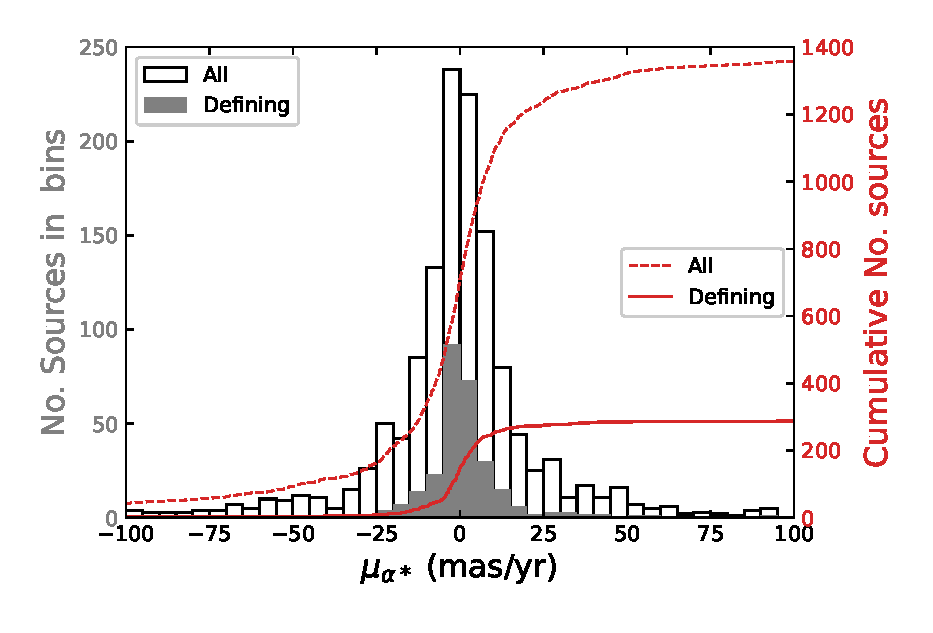
\includegraphics[width=\columnwidth]{figs/pmra-hist-glo}
        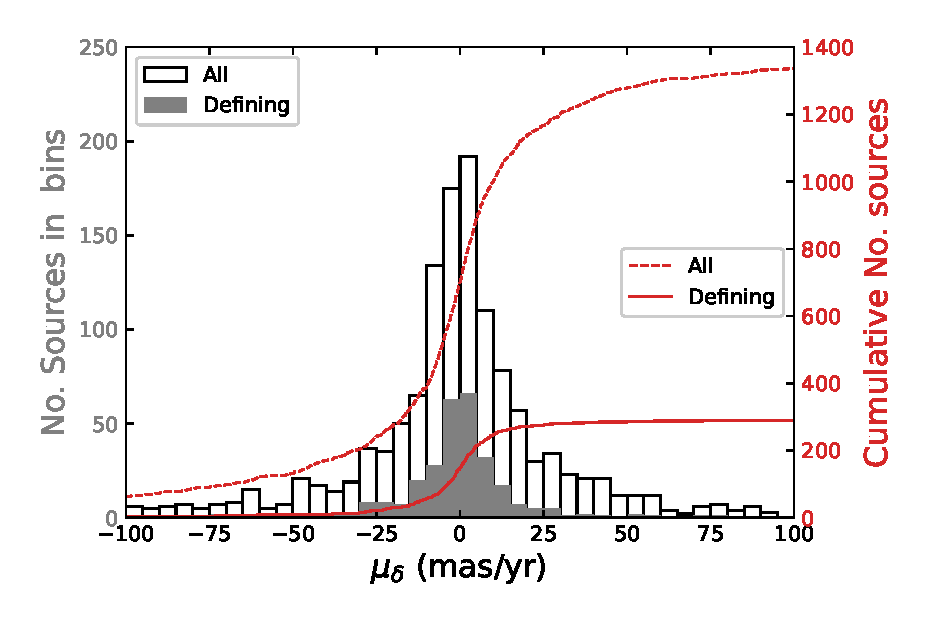
\includegraphics[width=\columnwidth]{figs/pmdec-hist-glo}
        \caption{Distribution of the apparent proper motion in the right ascension ($left$) and declination ($right$) for 1006 radio sources fitted from their coordinate time series.
            The left and right vertical axes indicates the number of sources in the each bin and cumulative from the leftmost bin.
            The distribution for 290 sources among the so-called 303 ICRF3 defining source list were labelled in different markers.}
    \end{figure}


%______________________________________________ Spin from APM
    \begin{figure}
        \label{fig:spin-dist}%  
        \centering
        % 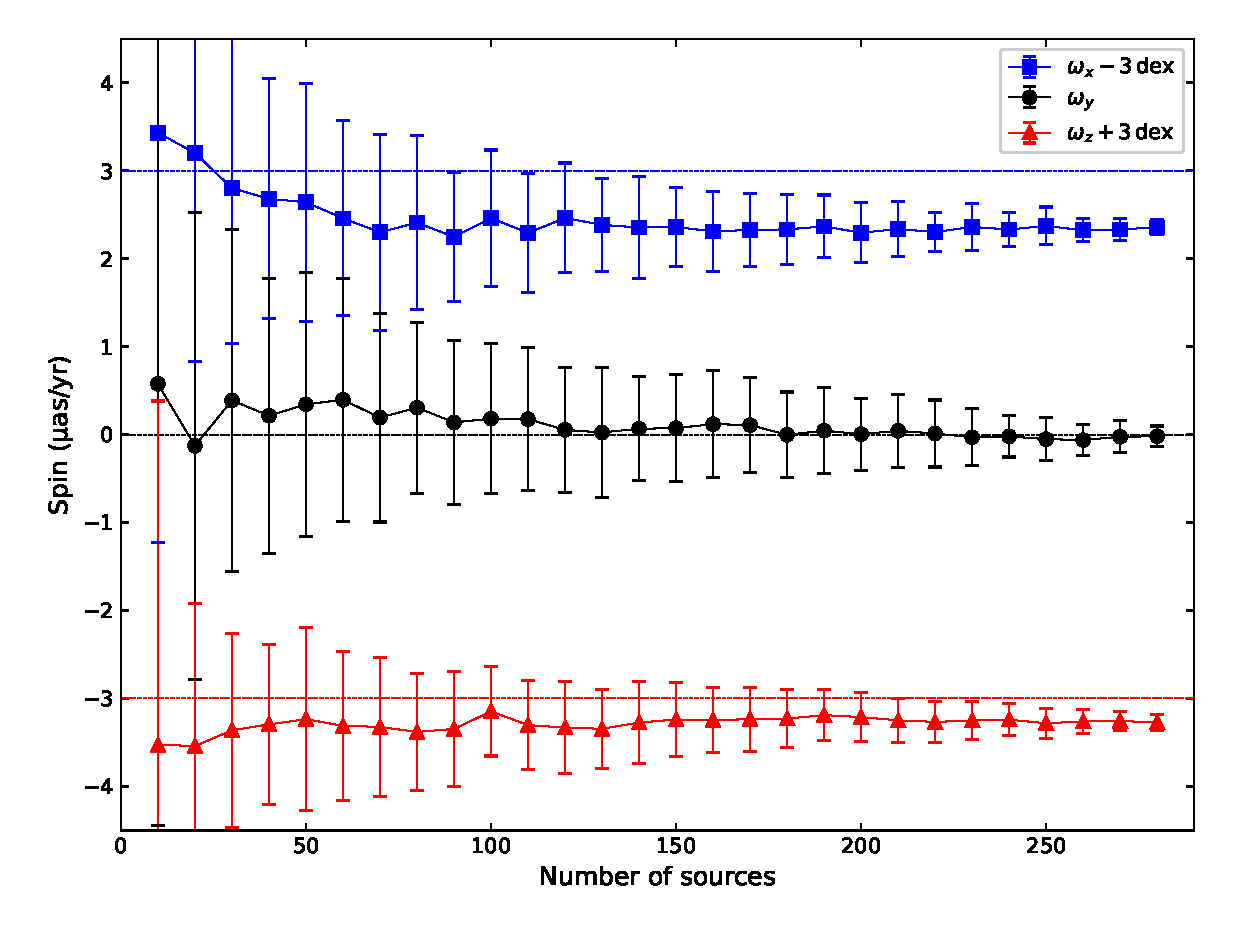
\includegraphics[width=\columnwidth]{figs/spin-from-apm}
        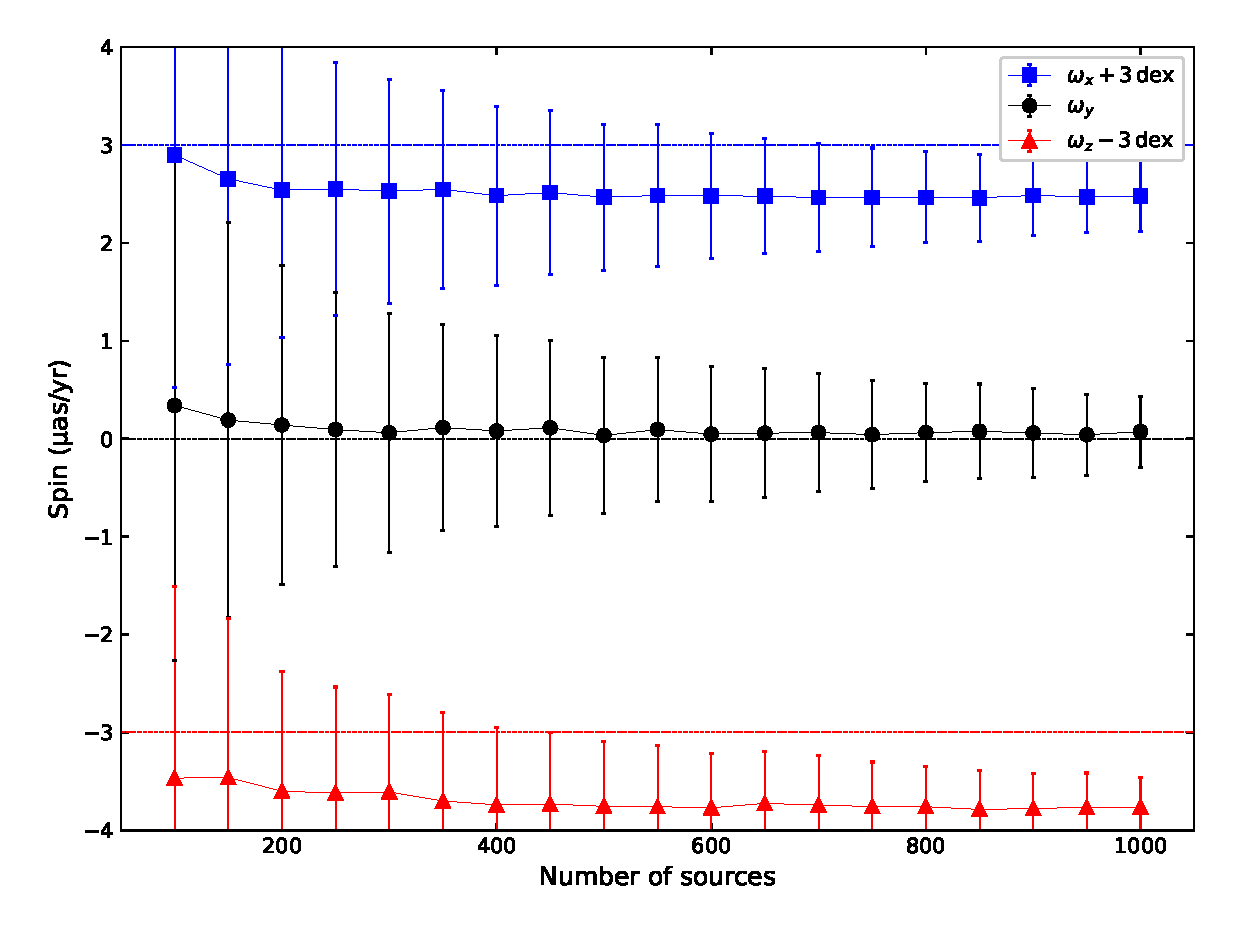
\includegraphics[width=\columnwidth]{figs/spin-from-apm-glo}
        \caption{
        Global spin estimated from the apparent proper motion versus the sample size used in the bootstrap sampling.
        The markers and errorbars stand for the mean value and standard deviation from 1000 bootstrap samples, respectively.
        }
    \end{figure}

    
    \textbf{
    % We obtained the apparent proper motion for 1484 sources, 290 sources being classified as the so-called ICRF3 defining source.
    The median value of the apparent proper motion for all sources is $\mathrm{0.18~\mu as\,yr^{-1}}$ in the R.A. and $\mathrm{-0.03~\mu as\,yr^{-1}}$ in the decl., respectively; they are $\mathrm{-0.06~\mu as\,yr^{-1}}$ and $\mathrm{-0.13~\mu as\,yr^{-1}}$ for the ICRF3 defining source subset.
    For most sources ($\gtrsim$70\%) in the sample, the apparent proper motion is within $\mathrm{\pm\,30~\mu as\,yr^{-1}}$ either in the R.A. or the declination.}
    
    \textbf{We fitted the global spin from the apparent proper motion.
    We first considered the 290 sources among the ICRF3 defining source list, and the reported the result below.
    %
    \begin{equation} \label{eq:spin-from-def}
         \begin{array}{l}
             \omega_x = -0.77 \pm 0.32\,\mathrm{\mu as\,yr^{-1}}, \\
             \omega_y = +0.50 \pm 0.35\,\mathrm{\mu as\,yr^{-1}}, \\
             \omega_z = -0.54 \pm 0.25\,\mathrm{\mu as\,yr^{-1}}. \\
         \end{array}
    \end{equation}
    %  
    The total spin was estimated to be $\omega = 1.07 \pm 0.31\,\mathrm{\mu as\,yr^{-1}}$, pointing to the direction of ($\alpha\,=\,147\,\pm\,21\,^{\circ}$, $\delta\,=\,-30\,\pm\,15\,^{\circ}$).
    We then estimated the global spin from the whole sample using the bootstrap sampling as described in Sect.~\ref{subsec:bs-mathod}.
    The sample size $N$ varies from 100 to 1000, with a step of 100.
    Figure.~\ref{fig:spin-dist} presents the distribution of the mean spin (marker) and the standard deviation (errorbar) as a functions of $N$.
    We found that the spin parameters were generally stable around some certain values, i.e., $\mathrm{\omega_x\sim-0.70\,\mu as\,yr^{-1}}$,  $\mathrm{\omega_y\sim-0.20\,\mu as\,yr^{-1}}$, and  $\mathrm{\omega_z\sim-0.55\,\mu as\,yr^{-1}}$.}
    
    \textbf{By taking the global spin value of $\mathrm{\sim 0.8\,\mu as\,yr^{-1}}$ and considering the time span of 41.6\,yr long (1979.6-2021.2), the accumulated deformation (orientation angle) in either axis of the VLBI celestial reference frame is about $\mathrm{33\,\mu as}$.
    This gives a rather conservation estimate of the ICRF axis stability since the global spin could be indeed smaller, for example, for the X- and Y-axis when considering the formal uncertainty.}

%______________________________________________________________

\subsection{Orientation of yearly CRFs relative to the ICRF3}  \label{subsec:orient-from-yearly-crf}
    
%______________________________________________ Rotation of yearly solution
    \begin{figure}
        \centering
        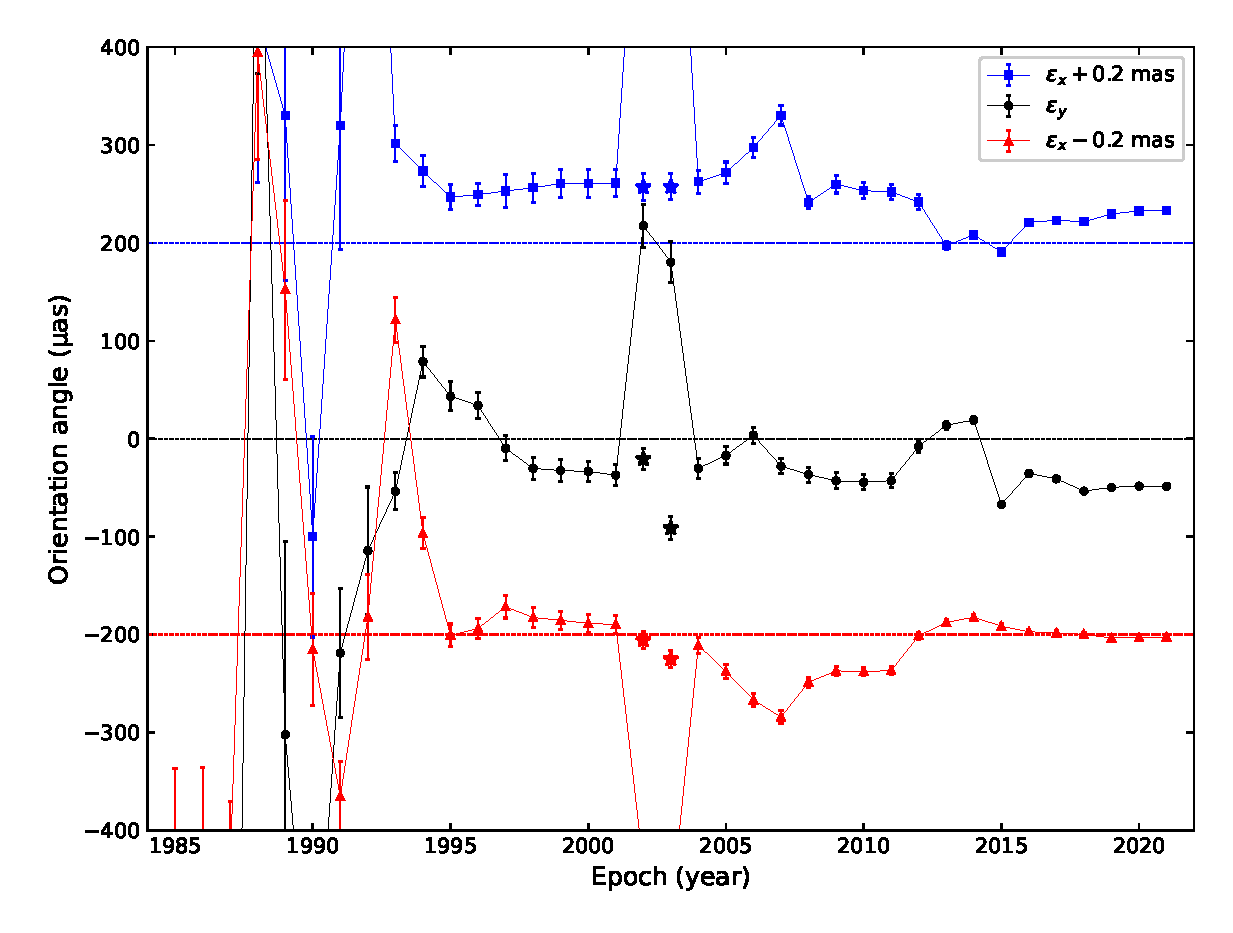
\includegraphics[width=\columnwidth]{figs/orient-from-yearly-solution}
        \caption{\label{fig:rot-yearly-sol}
        Orientation of yearly celestial references constructed from the VLBI global solution with respect to the ICRF3 $S/X$-band catalog based on the ICRF3 defining source subset. 
        The horizontal axis represents the epoch to whose beginning the VLBI observations were truncated at.
        The asterisks markers the results from two VLBI global solutions where the source 1004-500 was removed from the list of sources used to maintain the celestial reference frame.
            }
    \end{figure}
    
    % 
%______________________________________________ Rotation of averaged time series
    \begin{figure}
        \centering
        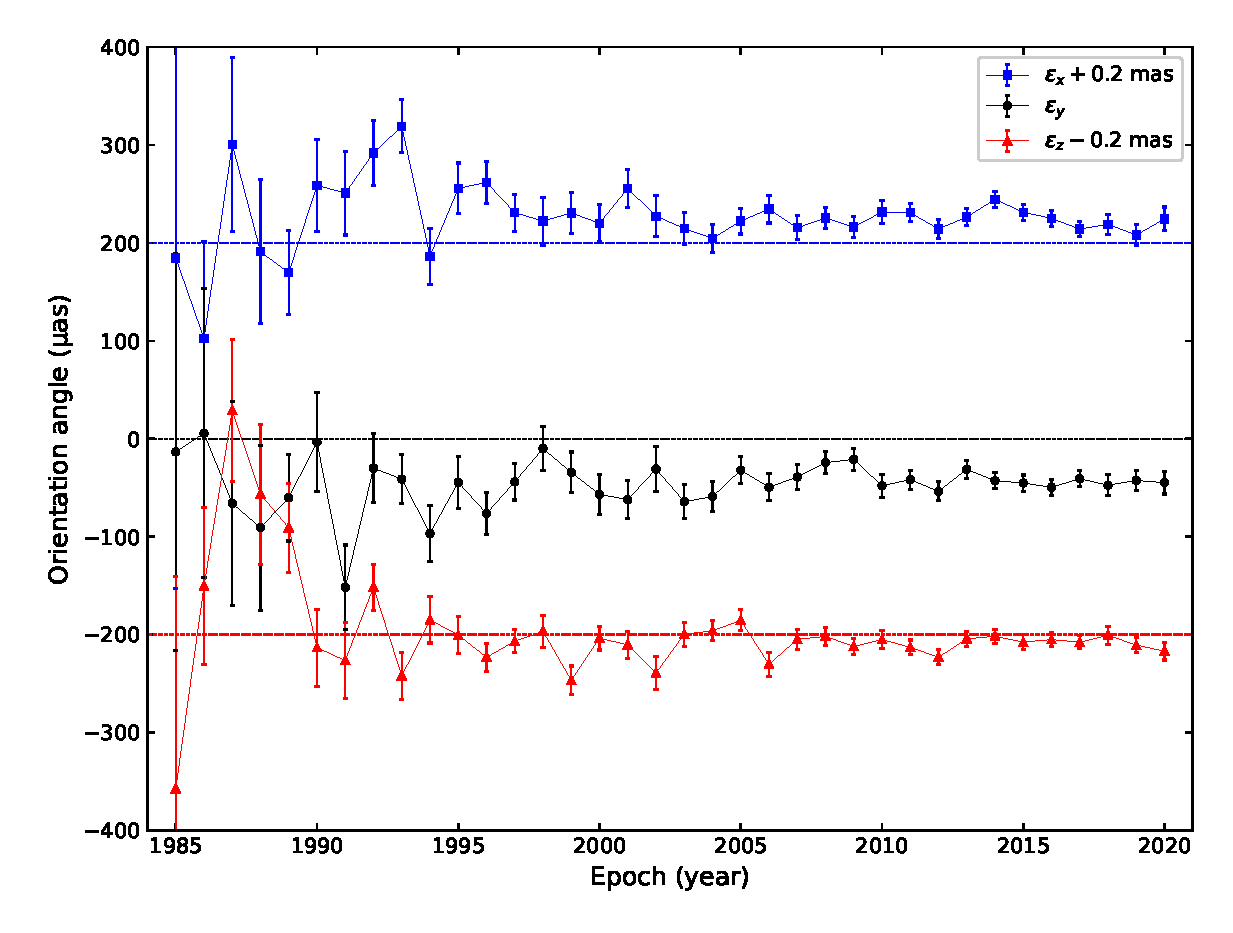
\includegraphics[width=\columnwidth]{figs/orient-from-yearly-ts-glo}
        \caption{\label{fig:rot-yearly-ts}   
         Orientation of yearly celestial references averaged from the coordinate time series with respect to the ICRF3 $S/X$-band catalog based on the ICRF3 defining source subset. 
         }
    \end{figure}
    
    % \textcolor{red}{}
    
    Figure~\ref{fig:rot-yearly-sol} depicts the orientation of the yearly celestial reference frames from the VLBI solutions with respect to the ICRF3 $S/X$-band catalog.
    The dispersion of the orientation angle reduces significantly after 1995, especially after 2015 which is the reference epoch of the ICRF3 catalog, except abrupt changes in 2002 and 2003 which are at the level of 0.2\,mas.
    \textbf{To figure out the possible origin, we compared the subsets of sources among the ICRF3 defining source ensemble in 2001 and in 2002.
    We found that an ICRF3 defining source 1004-500 was first observed on June 06, 2001 (session name: \texttt{01JUN06XN}) but only with one usable observations, which leaded to an estimate of position for this source with an formal uncertainty of $\sim$100\,mas and deviation of $\sim$50\,mas to its ICRF3 $S/X$-band position (in 2001 and 2002).
    This source was re-observed in 2003 in five sessions with the usable observation increased to 14, improving the formal uncertainty in source position to be better than 1\,mas (in 2004).
    When removing this source from the subset of sources used to maintain the celestial reference frame and re-ran the global solutions, the relative orientations of the new solutions with respect to the ICRF3 were significantly reduced at 2002 and 2003, as shown by the asterisks in Fig.~\ref{fig:rot-yearly-sol}.
    One can still see an orientation $\mathrm{\epsilon_y\sim-0.1\,mas}$ at 2003, which can be easily explained by the inclusion of new ICRF3 defining source 0038-326 with few observations (nine) and thus a poor position estimated precision ($\mathrm{\sim12\,mas}$).
    Again, removing this source together with 1004-500 from the CRF maintaining source list would further reduce $\mathrm{\epsilon_y}$ to several tens of $\mathrm{\mu as}$.
    We also noted that the source 0038-326 were no longer observed until 2011 but $\mathrm{\epsilon_y}$ is stable at around $\mathrm{30\,\mu as}$ in the period of 2004-2010.
    The possible reason could be that more new ICRF3 defining sources entered to enhance the celestial frame during this period, which diminished the influence of 0038-326.
    }
    
    The weighted mean value of the orientation angle is $\mathrm{+26\,\mu as}$, $\mathrm{-41\,\mu as}$, and $\mathrm{-4\,\mu as}$ for the X-, Y-, and Z-axis, respectively.
    The corresponding standard deviations are $\mathrm{22\,\mu as}$, $\mathrm{24\,\mu as}$, and $\mathrm{22\,\mu as}$.
    If removing these data points before 1995 and at 2002-2003, the mean values change little whereas the standard deviations were reduced to $\mathrm{16\,\mu as}$, $\mathrm{19\,\mu as}$, and $\mathrm{16\,\mu as}$.
    
    Similarly, the relative orientation angles of the yearly celestial frame based on the coordinate time series become more stable after around 1995 as shown in Fig.~\ref{fig:rot-yearly-ts}.
    The weighted mean value and standard deviation of the orientation angle around the X-, Y-, and Z-axis are $\mathrm{+26\,\pm\,16\,\mu as}$, $\mathrm{-43\,\pm\,13\,\mu as}$, and $\mathrm{-8\,\pm\,14\,\mu as}$, respectively.
    When only considering the data points after 1995, the corresponding standard deviations were reduced to $\mathrm{10\,\mu as}$.
    
    Generally, the relative orientation angles shown in the Fig.~\ref{fig:rot-yearly-sol} and Fig.~\ref{fig:rot-yearly-ts} are consistent with the formal uncertainty (error bars).
    In short, the axis of the yearly celestial reference frame is stable at the level of $\mathrm{10-20\,\mu as}$.
    
    
%______________________________________________________________

\subsection{Orientation of various radio catalogs relative to the ICRF3}  \label{subsec:orient-from-ivs-sol}    
    
%__________________________________________________ One column table

\begin{table}
    \caption{Relative orientation of various catalogs with referred to the ICRF3 $S/X$ catalogs based on the subset of ICRF3 defining sources.}
    \label{tab:orient-def}
    $$
    \begin{tabular}{cccccccc}
        \hline
        \noalign{\smallskip}
        Catalog     &\epsilon_x & \pm &\epsilon_y & \pm &\epsilon_z & \pm  \\
        \hline
        \noalign{\smallskip}
        asi2020a    & $-$4  & 3     & +5   & 2      &  +5   & 1 \\
        aus2020b    & $-$4  & 3     & +0   & 3      & $-$9  & 3 \\
        % opa2019a    & +25   & 1     &$-$52 & 1      & $-$1  & 1 \\
        opa2021a    & +36   & 4     &$-$52 & 4      & $-$10  & 3 \\
        usn2019c    & +2    & 1     & +0   & 1      & +12   & 1 \\
        ICRF2       & +14   & 6     & +14   & 6     & $-$4  & 5 \\
        \noalign{\smallskip}
        \hline
        \noalign{\smallskip}
        ICRF3 $K$   & $-$3  & 11    & $-$15 & 11    & $-$7  & 7 \\
        ICRF3 $X/Ka$& $-$6  & 20    & $-$11 & 21    & +28   & 15 \\
        \hline
        \noalign{\smallskip}
    \end{tabular}
    $$
    \tablefoot{The orientation angle ($\epsilon_x$, $\epsilon_y$, $\epsilon_z$) and the formal uncertainty ($\pm$) are estimated by the mean and standard deviation.}
\end{table}


    Table~\ref{tab:orient-def} reports the relative orientation of various radio catalogs
    % with similar amount of data but different analysis strategies 
    with referred to the ICRF3 $S/X$-band catalogs based on the subset of the ICRF3 defining sources.
    These orientation angles are generally less than $\mathrm{10\,\mu as}$, except for opa2021a.
    When comparing the ICRF2 with the ICRF3 $S/X$-band catalogs, the orientation angle is also on the order of $\mathrm{10\,\mu as}$.
    As a result, the difference in the axis direction between celestial reference frames represented by different catalogs at $S/X$-band is generally on the level of $\mathrm{10\,\mu as}$.
    
    We compared the relative orientation of representations of the ICRF3 at three bands.
    The orientation offset is about $\mathrm{10\,\mu as}$, except for the Y-axis between the $K$-band and $S/X$-band, and the Z-axis between the $X/Ka$-band and $S/X$-band.

%______________________________________________________________

\subsection{Orientation agreement among different realizations of ICRS}  \label{subsec:axis-agreement}  

\begin{table}
    \caption{Orientation agreement among realizations of the ICRS at different wavelengths.}
    \label{tab:orient-all}
    $$
    \begin{tabular}{ccccccccc}
        \hline
        \noalign{\smallskip}
        Catalog     &$N$ &\epsilon_x & \pm &\epsilon_y & \pm &\epsilon_z & \pm  \\
        \hline
        \noalign{\smallskip}
        wrt. ICRF3 $S/X$ & &&&&&& \\
        ICRF2       & 2300 & $  +9$ &   3 & $ +14$ &   3 & $  -2$ &   2 \\
        ICRF3 $K$   & 550  & $ -11$ &   5 & $ -18$ &   4 & $  -7$ &   3 \\
        ICRF3 $X/Ka$& 450  & $ -17$ &   7 & $  -2$ &   7 & $ +49$ &   5 \\
        \noalign{\smallskip}
        \hline
        \noalign{\smallskip}
        wrt. \textit{Gaia} EDR3 & &&&&&& \\
        ICRF3 $S/X$ & 2100 & $  -2$ & 5 & $  -2$ & 5 & $  -2$ & 5 \\
        ICRF3 $K$   & 440 & $ -12$ & 14 & $ -12$ & 14 & $ -12$ & 14 \\
        ICRF3 $X/Ka$& 384 & $  -8$ & 20 & $  -8$ & 20 & $  -8$ & 20 \\
        \hline
        \noalign{\smallskip}
    \end{tabular}
    $$
    \tablefoot{The orientation angle ($\epsilon_x$, $\epsilon_y$, $\epsilon_z$) and the formal uncertainty ($\pm$) are estimated by the mean and standard deviation.}
\end{table}
    
    In order to assess the overall agreement in the axial directions of different realizations of the ICRS, we adopted the bootstrap sampling method as described in Sect.~\ref{subsec:bs-mathod} and presented the results in Table~\ref{tab:orient-all}.
    About two thirds of the whole common sources were picked in each iteration.
    The ICRF3 $S/X$ catalogs were used as the reference catalog, in which case we assessed the internal alignment precision of the ICRF3.
    We found that the scatter (standard deviation) of relative orientation of the ICRF2, ICRF3 $K$-band, and ICRF3 $X/Ka$-band is all smaller than $\mathrm{7\,\mu as}$, despite the constant orientation offset.
    It suggested that the internal alignment precision is on the level of $\mathrm{7\,\mu as}$ or better.
    
    We also evaluated the potential precision of the VLBI-\textit{Gaia} frame link by setting the \textit{Gaia} EDR3 position as the reference.
    The agreement in the axis orientation is about $\mathrm{5\,\mu as}$ between the ICRF3 $S/X$-band and \textit{Gaia} EDR3, $\mathrm{14\,\mu as}$ for the $K$-band, and $\mathrm{20\,\mu as}$ for the $X/Ka$-band.
    Considering that the \textit{Gaia} measurement precision and accuracy will be both continuously improved and so do the VLBI celestial reference frames,
    these values could be considered as a conservation estimate of the alignment precision that the future radio-to-optical frame link can achieve.

%
%                                                One column figure
%----------------------------------------------------------- S_vib
%   \begin{figure}
%   \centering
%   \includegraphics[width=3cm]{figure.pdf}
%       \caption{Vibrational stability equation of state
%               $S_{\mathrm{vib}}(\lg e, \lg \rho)$.
%               $>0$ means vibrational stability.
%               }
%          \label{FigVibStab}
%   \end{figure}
%
%______________________________________________________________

\section{Conclusions}

    % Two conclusions might be drawn.
   \begin{enumerate}
      \item The stability of the ICRF axes is found to be about $\mathrm{10}$-$\mathrm{20\,\mu as}$, depending on the methods used.
      \item The internal alignment precision of the ICRF3 is on the level of $\mathrm{10}$-$\mathrm{20\,\mu as}$.
      \item The potential precision for the optical-to-radio frame link is no worse than $\mathrm{20\,\mu as}$ and can reach $\mathrm{5\,\mu as}$ for the $S/X$-band ICRF and the \textit{Gaia}-CRF.
   \end{enumerate}

\begin{acknowledgements}
      
\end{acknowledgements}

\bibliographystyle{aa} % style aa.bst
\bibliography{references} % your references Yourfile.bib

\begin{appendix} %First online appendix

\section{Glide estimate}

The glide parameters of the yearly CRFs wrt. the ICRF3 $S/X$-band frame are presented in Figs.~\ref{fig:gli-yearly-sol}-\ref{fig:gli-yearly-ts}, corresponding to Figs.~\ref{fig:rot-yearly-sol}-\ref{fig:rot-yearly-ts}.

%______________________________________________ glide of yearly solution
    \begin{figure}
        \centering
        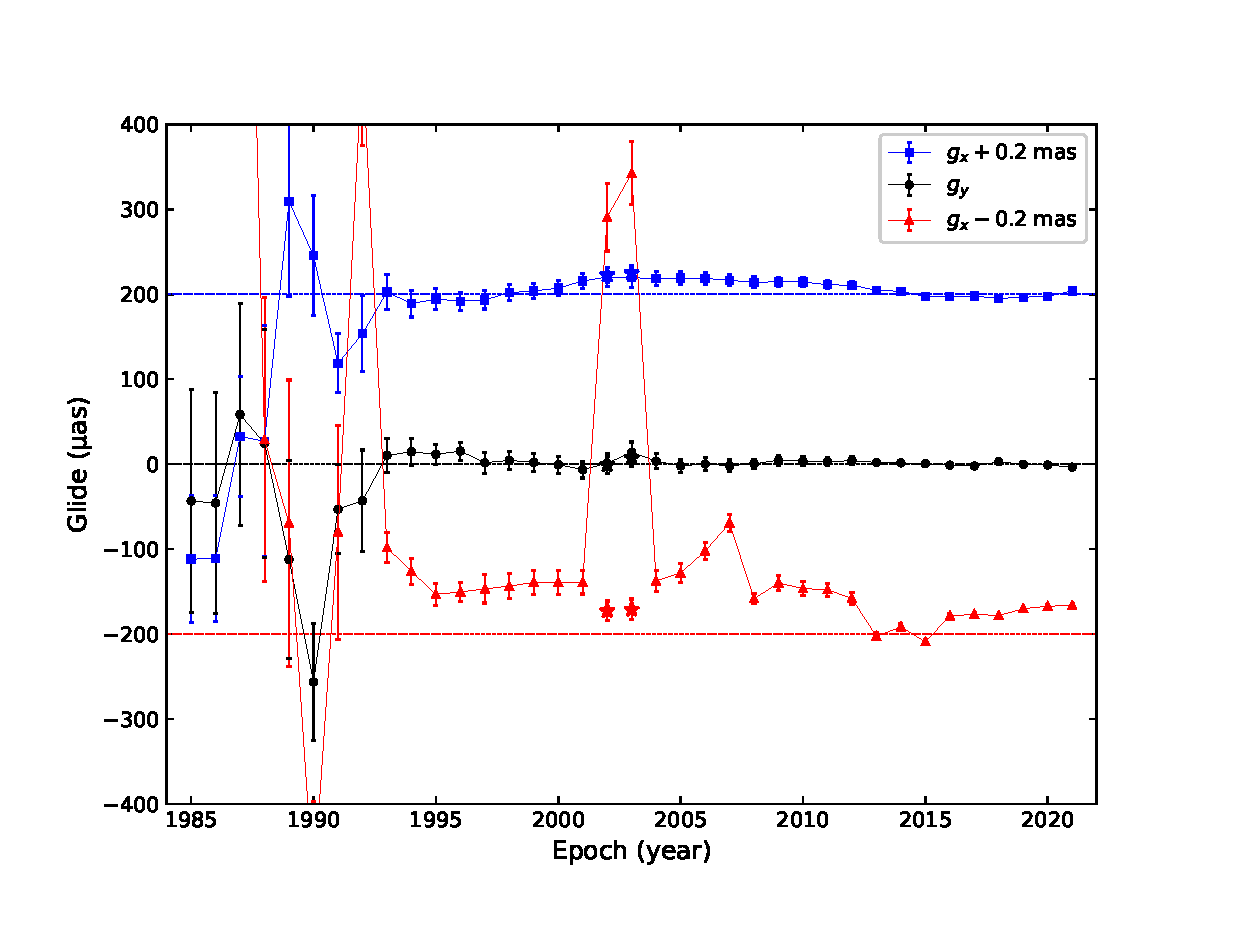
\includegraphics[width=\columnwidth]{figs/glide-from-yearly-solution}
        \caption{\label{fig:gli-yearly-sol}
        Glide of yearly celestial references constructed from the VLBI global solution with respect to the ICRF3 $S/X$-band catalog based on the ICRF3 defining source subset. 
        The horizontal axis represents the epoch to whose beginning the VLBI observations were truncated at.
        The asterisks markers the results from two VLBI global solutions where the source 1004-500 was removed from the list of sources used to maintain the celestial reference frame.
            }
    \end{figure}
    
    % 
%______________________________________________ glide of averaged time series
    \begin{figure}
        \centering
        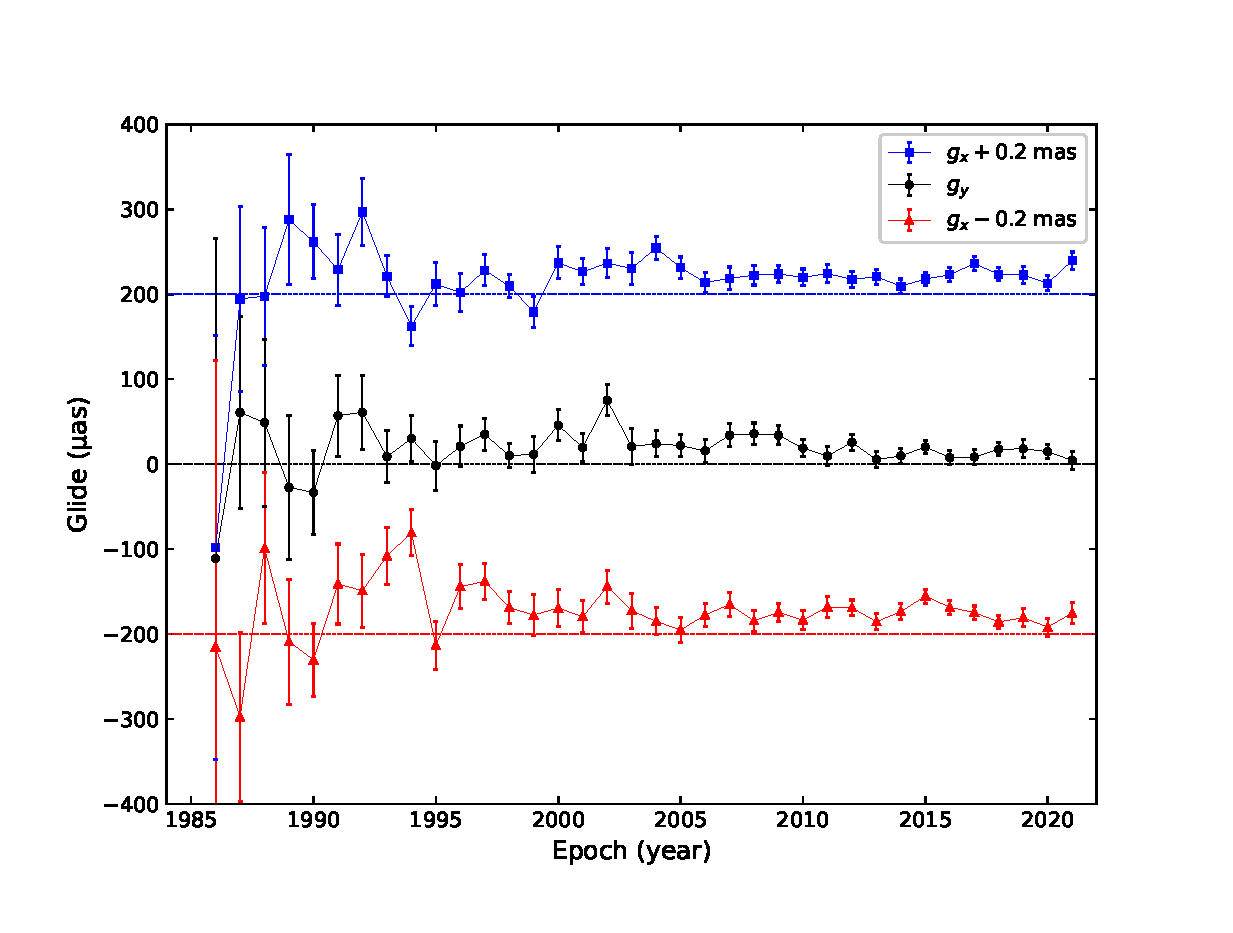
\includegraphics[width=\columnwidth]{figs/glide-from-yearly-ts-glo}
        \caption{\label{fig:gli-yearly-ts}   
         Glide of yearly celestial references averaged from the coordinate time series with respect to the ICRF3 $S/X$-band catalog based on the ICRF3 defining source subset. 
         }
    \end{figure}


\section{Orientation agreements of various VLBI solutions} %Second online appendix

\begin{table}
    \caption{Orientation agreement among realizations of the ICRS by various IVS radio source catalogs.}
    \label{tab:orient-all}
    $$
    \begin{tabular}{cccccccccc}
        \hline
        \noalign{\smallskip}
        Catalog     &$N_{\rm com}$ &$N_{\rm used}$ &\epsilon_x & \pm &\epsilon_y & \pm &\epsilon_z & \pm  \\
        \hline
        \noalign{\smallskip}
        % wrt. ICRF3 $S/X$ & &&&&&& \\
        opa2021a & 4490 & 3000 & $ +34$ & 3 & $ -50$ & 3 & $  -8$ & 4 \\
        asi2020a & 4296 & 3000 & $  -2$ & 2 & $  +7$ & 2 & $  +7$ & 1 \\
        aus2020b & 4456 & 3000 & $ -15$ & 7 & $  +4$ & 4 & $  -7$ & 3 \\
        usn2019c & 2263 & 1500 & $  +3$ & 1 & $  -0$ & 1 & $ +13$ & 1 \\
        \hline
        \noalign{\smallskip}
    \end{tabular}
    $$
    \tablefoot{The orientation angle ($\epsilon_x$, $\epsilon_y$, $\epsilon_z$) and the formal uncertainty ($\pm$) are estimated by the mean and standard deviation.}
\end{table}


\section{Session-wise CRFs} %Second online appendix

The source positions derived from observations in each sessions solely were
drawn from the \texttt{.lso} file available at the Paris Observatory Geodetic VLBI Center 
\footnote{\url{http://ivsopar.obspm.fr/radiosources/opa2021r.lso}}, which contains estimate of 
source positions from session-wise independent VLBI solution, and we used 
these position to form the session-wise celestial reference frame.
Then I estimated the rotation and glide parameters of these session-wise CRFs with respect to 
the ICRF3 based on the subset of sources common to the ICRF3 defining source ensemble
(I also considered using all common sources to the ICRF3 but the results are not presented here).
Source whose position difference between the session-wise CRF and ICRF3 $S/X$ is greater than 10~mas 
or is three times greater than their formal uncertainty was removed.
Only sessions with more than six sources common to the ICRF3 defining source ensemble were considered, 
which rejected most sessions before the 1990
Figure~\ref{fig:sess-wise-pmt} presents the estimates of rotation and glide parameters.
I also computed the root-mean-square of every 100 data points weighted by their formal uncertainties 
as the scatter of the parameters, as indicated by the red dashed line therein.
The rotation parameters are generally stable at the level of 100-200~$\mathrm{\mu as}$ since 1995, except a small jump in $\epsilon_x$ and $\epsilon_y$ at about 2017.
A similar jump can also be seen in $g_z$.
So one may say that the ICRF3 stability is satisfied among 1990 (or 1979)-2021.


%% {fig:waterfalls}
%===========================================================================
 \begin{figure}[hbtp]
   \centering
   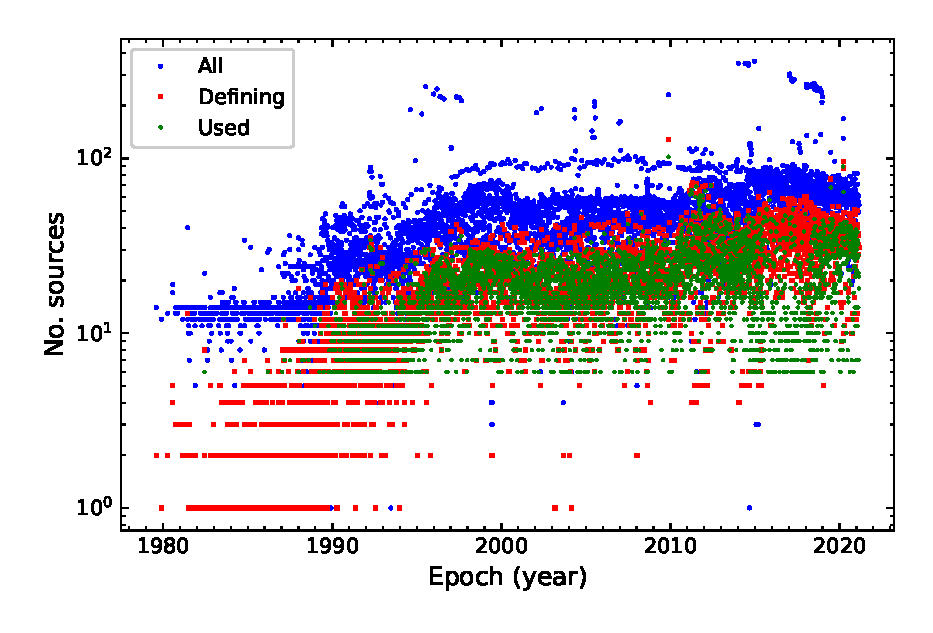
\includegraphics[width=\columnwidth]{figs/num_sou_in_sess}  %% no file extension
   \caption[]{\label{fig:waterfalls} %
	Number of sources in session-wise radio source catalogs.
	The numbers of all sources, sources among the ICRF3 defining source list, and
	sources actually used to estimate the rotation and glide are shown in different markers.
   }
 \end{figure}
% ===========================================================================
%% Have "floats" such as figures between blank lines to make them float



%% {fig:waterfalls}
%===========================================================================
 \begin{figure*}[hbtp]
   \centering
   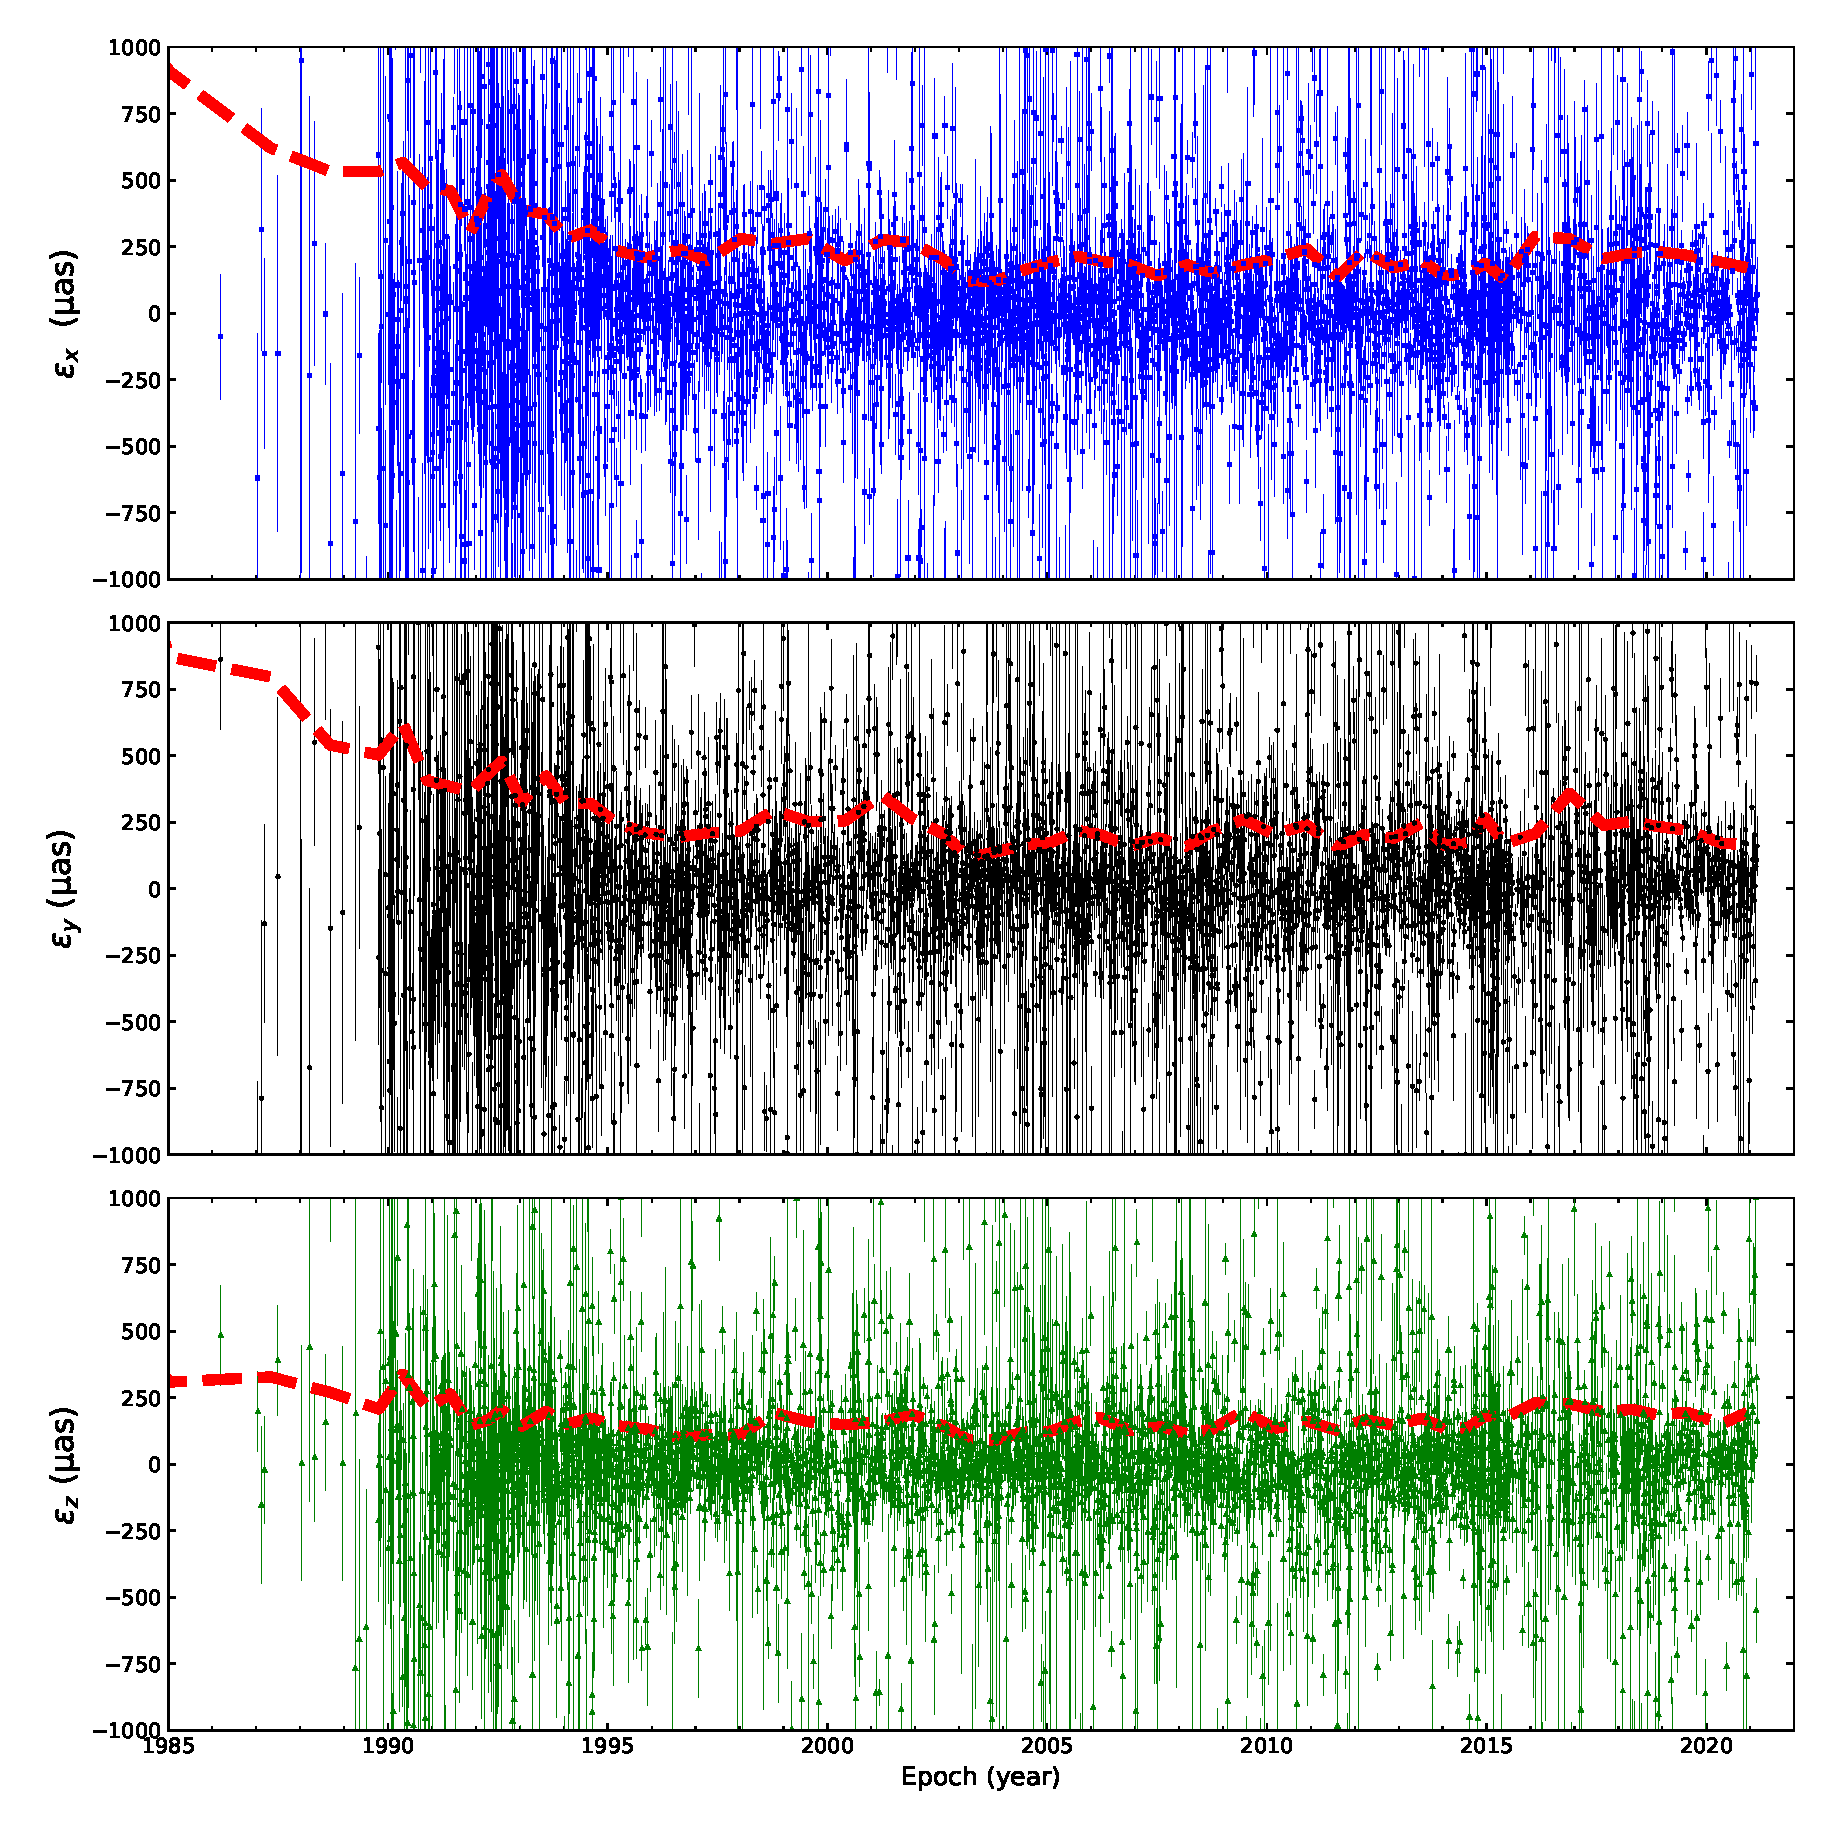
\includegraphics[width=\columnwidth]{figs/orient-from-sess-crf}  %% no file extension
   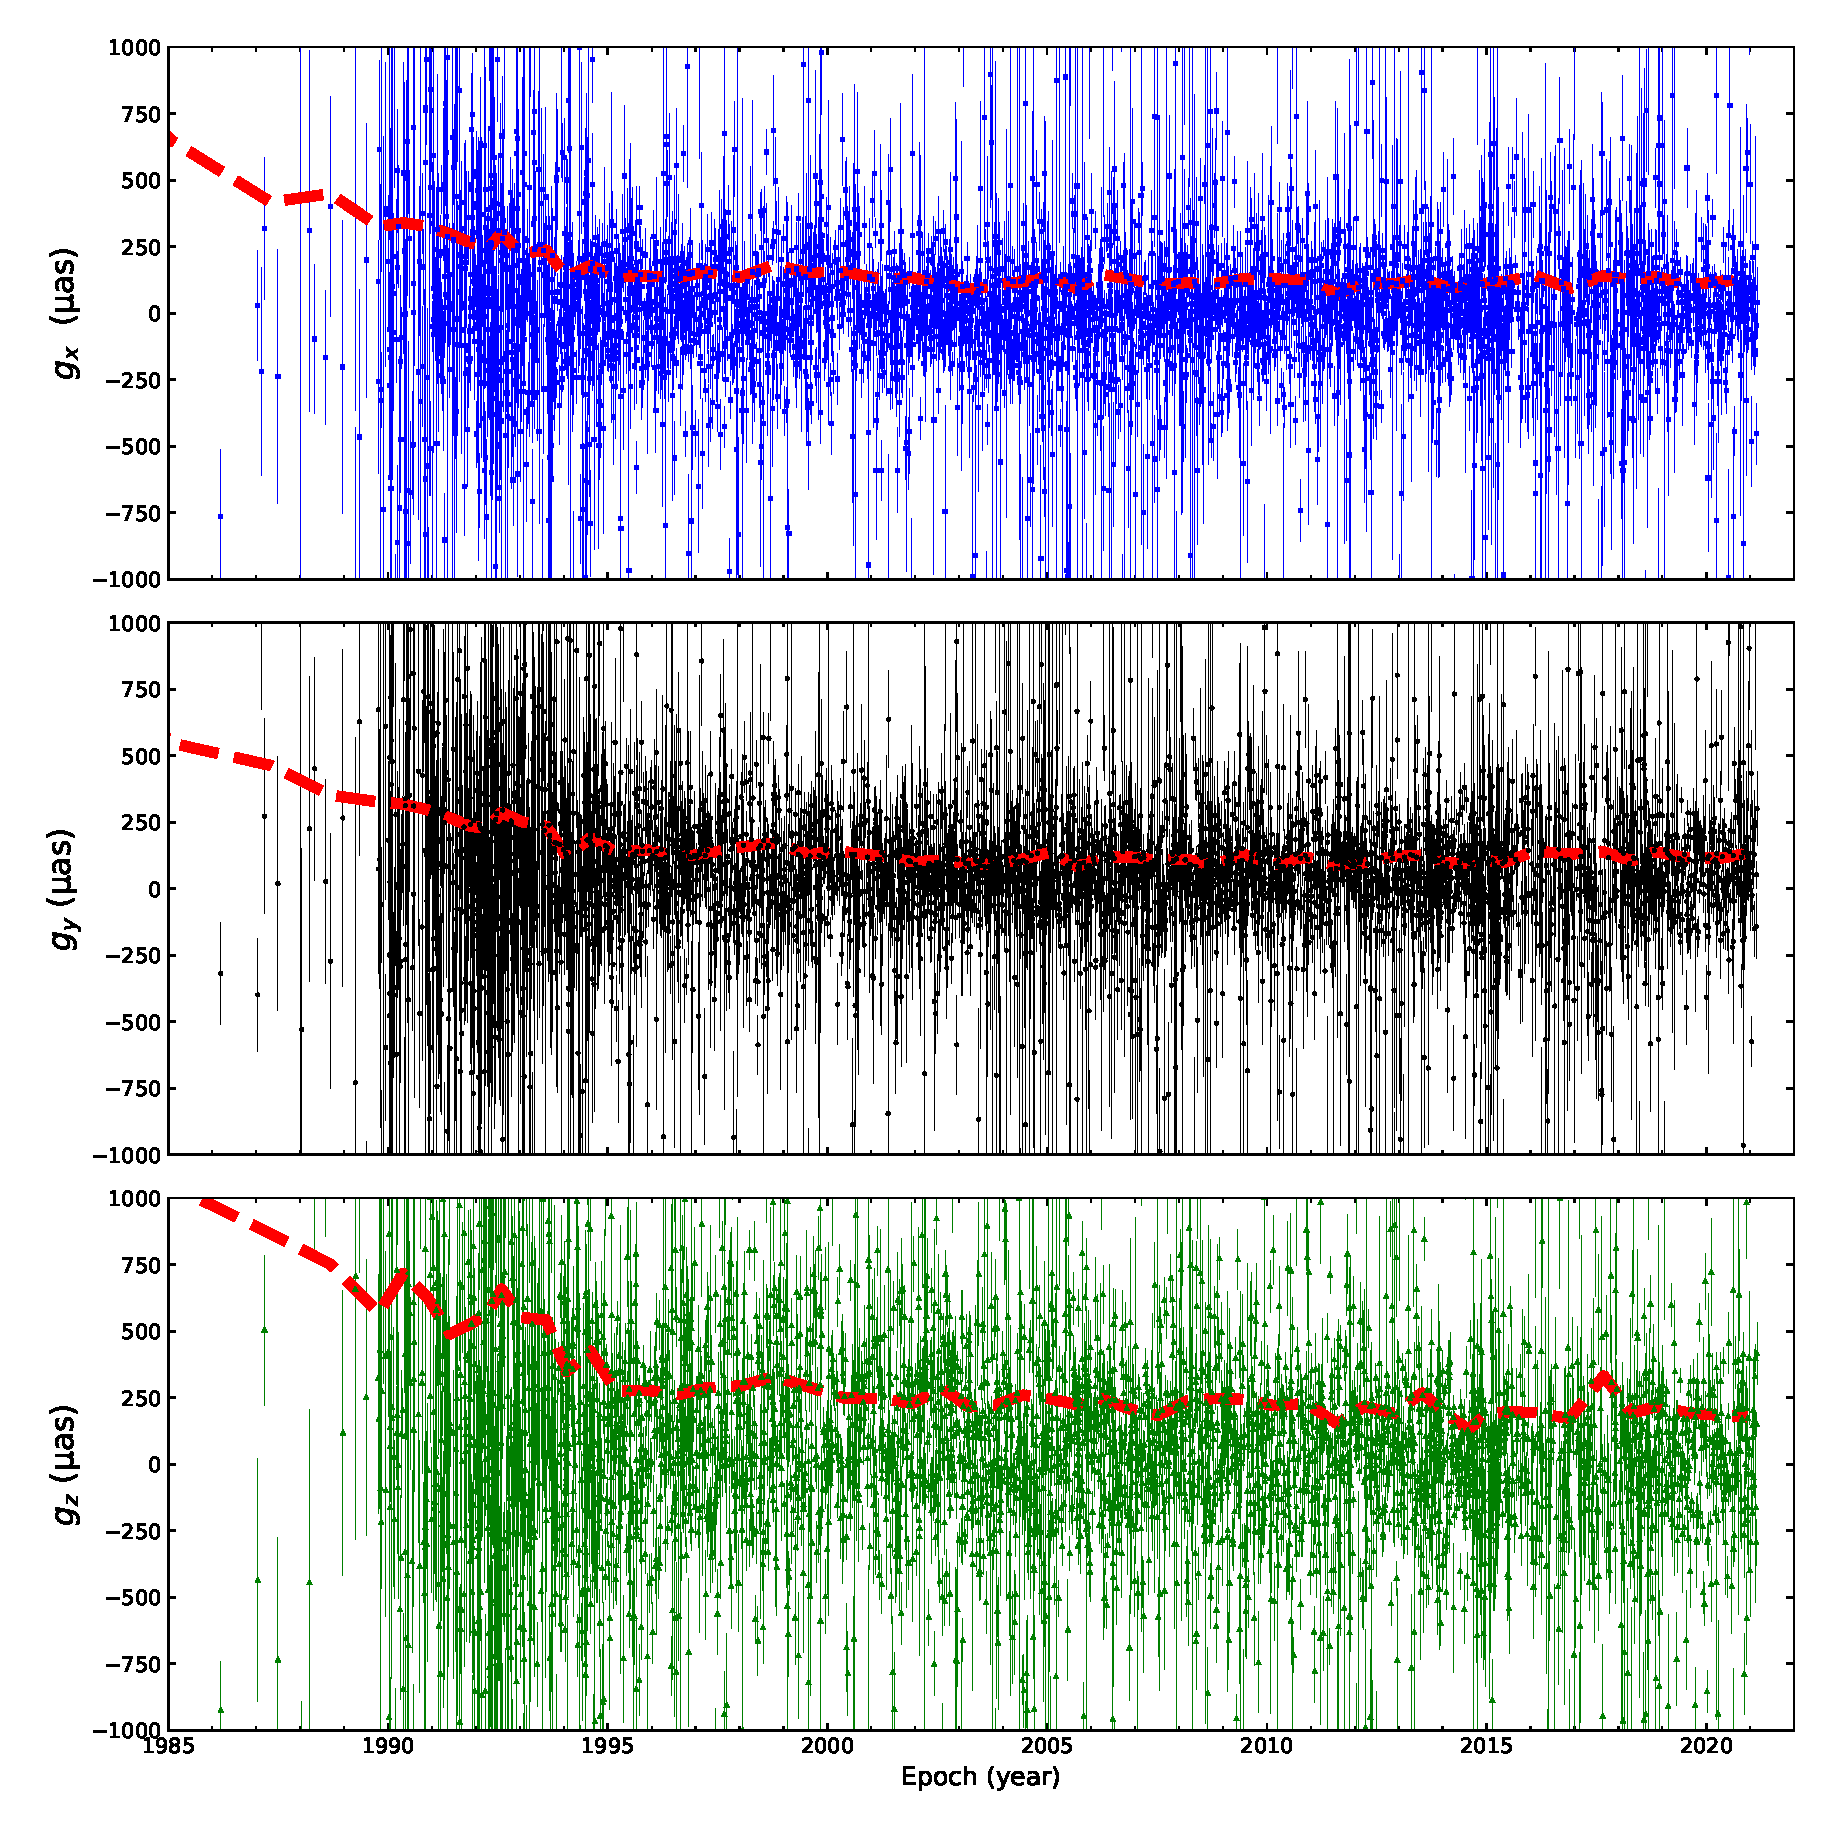
\includegraphics[width=\columnwidth]{figs/glide-from-sess-crf}  %% no file extension
   \caption[]{\label{fig:sess-wise-pmt} %
	Rotation ($left$) and glide ($right$) of session-wise CRFs with referred to
	the ICRF3 $S/X$-band catalog.
	The formal uncertainty of parameter estimate is indicated by the errorbar.
	The red dashed line shows the weighted root-mean-square (wrms) of every 100 points.
   }
 \end{figure*}
% ===========================================================================

\end{appendix}

\end{document}
%% Below are further examples

%%%%%%%%%%%%%%%%%%%%%%%%%%%%%%%%%%%%%%%%%%%%%%%%%%%%%%%%%%%%%%
Examples for figures using graphicx
A guide "Using Imported Graphics in LaTeX2e"  (Keith Reckdahl)
is available on a lot of LaTeX public servers or ctan mirrors.
The file is : epslatex.pdf 
%%%%%%%%%%%%%%%%%%%%%%%%%%%%%%%%%%%%%%%%%%%%%%%%%%%%%%%%%%%%%%

%_____________________________________________________________
%                 A figure as large as the width of the column
%-------------------------------------------------------------
   \begin{figure}
   \centering
   \includegraphics[width=\hsize]{empty.eps}
      \caption{Vibrational stability equation of state
               $S_{\mathrm{vib}}(\lg e, \lg \rho)$.
               $>0$ means vibrational stability.
              }
         \label{FigVibStab}
   \end{figure}
%
%_____________________________________________________________
%                                    One column rotated figure
%-------------------------------------------------------------
   \begin{figure}
   \centering
   \includegraphics[angle=-90,width=3cm]{empty.eps}
      \caption{Vibrational stability equation of state
               $S_{\mathrm{vib}}(\lg e, \lg \rho)$.
               $>0$ means vibrational stability.
              }
         \label{FigVibStab}
   \end{figure}
%
%_____________________________________________________________
%                        Figure with caption on the right side 
%-------------------------------------------------------------
   \begin{figure}
   \sidecaption
   \includegraphics[width=3cm]{empty.eps}
      \caption{Vibrational stability equation of state
               $S_{\mathrm{vib}}(\lg e, \lg \rho)$.
               $>0$ means vibrational stability.
              }
         \label{FigVibStab}
   \end{figure}
%
%_____________________________________________________________
%
%_____________________________________________________________
%                                Figure with a new BoundingBox 
%-------------------------------------------------------------
   \begin{figure}
   \centering
   \includegraphics[bb=10 20 100 300,width=3cm,clip]{empty.eps}
      \caption{Vibrational stability equation of state
               $S_{\mathrm{vib}}(\lg e, \lg \rho)$.
               $>0$ means vibrational stability.
              }
         \label{FigVibStab}
   \end{figure}
%
%_____________________________________________________________
%
%_____________________________________________________________
%                                      The "resizebox" command 
%-------------------------------------------------------------
   \begin{figure}
   \resizebox{\hsize}{!}
            {\includegraphics[bb=10 20 100 300,clip]{empty.eps}
      \caption{Vibrational stability equation of state
               $S_{\mathrm{vib}}(\lg e, \lg \rho)$.
               $>0$ means vibrational stability.
              }
         \label{FigVibStab}
   \end{figure}
%
%______________________________________________________________
%
%_____________________________________________________________
%                                             Two column Figure 
%-------------------------------------------------------------
   \begin{figure*}
   \resizebox{\hsize}{!}
            {\includegraphics[bb=10 20 100 300,clip]{empty.eps}
      \caption{Vibrational stability equation of state
               $S_{\mathrm{vib}}(\lg e, \lg \rho)$.
               $>0$ means vibrational stability.
              }
         \label{FigVibStab}
   \end{figure*}
%
%______________________________________________________________
%
%_____________________________________________________________
%                                             Simple A&A Table
%_____________________________________________________________
%
\begin{table}
\caption{Nonlinear Model Results}             % title of Table
\label{table:1}      % is used to refer this table in the text
\centering                          % used for centering table
\begin{tabular}{c c c c}        % centered columns (4 columns)
\hline\hline                 % inserts double horizontal lines
HJD & $E$ & Method\#2 & Method\#3 \\    % table heading 
\hline                        % inserts single horizontal line
   1 & 50 & $-837$ & 970 \\      % inserting body of the table
   2 & 47 & 877    & 230 \\
   3 & 31 & 25     & 415 \\
   4 & 35 & 144    & 2356 \\
   5 & 45 & 300    & 556 \\ 
\hline                                   %inserts single line
\end{tabular}
\end{table}
%
%_____________________________________________________________
%                                             Two column Table 
%_____________________________________________________________
%
\begin{table*}
\caption{Nonlinear Model Results}             
\label{table:1}      
\centering          
\begin{tabular}{c c c c l l l }     % 7 columns 
\hline\hline       
                      % To combine 4 columns into a single one 
HJD & $E$ & Method\#2 & \multicolumn{4}{c}{Method\#3}\\ 
\hline                    
   1 & 50 & $-837$ & 970 & 65 & 67 & 78\\  
   2 & 47 & 877    & 230 & 567& 55 & 78\\
   3 & 31 & 25     & 415 & 567& 55 & 78\\
   4 & 35 & 144    & 2356& 567& 55 & 78 \\
   5 & 45 & 300    & 556 & 567& 55 & 78\\
\hline                  
\end{tabular}
\end{table*}
%
%-------------------------------------------------------------
%                                          Table with notes 
%-------------------------------------------------------------
%
% A single note
\begin{table}
\caption{\label{t7}Spectral types and photometry for stars in the
  region.}
\centering
\begin{tabular}{lccc}
\hline\hline
Star&Spectral type&RA(J2000)&Dec(J2000)\\
\hline
69           &B1\,V     &09 15 54.046 & $-$50 00 26.67\\
49           &B0.7\,V   &*09 15 54.570& $-$50 00 03.90\\
LS~1267~(86) &O8\,V     &09 15 52.787&11.07\\
24.6         &7.58      &1.37 &0.20\\
\hline
LS~1262      &B0\,V     &09 15 05.17&11.17\\
MO 2-119     &B0.5\,V   &09 15 33.7 &11.74\\
LS~1269      &O8.5\,V   &09 15 56.60&10.85\\
\hline
\end{tabular}
\tablefoot{The top panel shows likely members of Pismis~11. The second
panel contains likely members of Alicante~5. The bottom panel
displays stars outside the clusters.}
\end{table}
%
% More notes
%
\begin{table}
\caption{\label{t7}Spectral types and photometry for stars in the
  region.}
\centering
\begin{tabular}{lccc}
\hline\hline
Star&Spectral type&RA(J2000)&Dec(J2000)\\
\hline
69           &B1\,V     &09 15 54.046 & $-$50 00 26.67\\
49           &B0.7\,V   &*09 15 54.570& $-$50 00 03.90\\
LS~1267~(86) &O8\,V     &09 15 52.787&11.07\tablefootmark{a}\\
24.6         &7.58\tablefootmark{1}&1.37\tablefootmark{a}   &0.20\tablefootmark{a}\\
\hline
LS~1262      &B0\,V     &09 15 05.17&11.17\tablefootmark{b}\\
MO 2-119     &B0.5\,V   &09 15 33.7 &11.74\tablefootmark{c}\\
LS~1269      &O8.5\,V   &09 15 56.60&10.85\tablefootmark{d}\\
\hline
\end{tabular}
\tablefoot{The top panel shows likely members of Pismis~11. The second
panel contains likely members of Alicante~5. The bottom panel
displays stars outside the clusters.\\
\tablefoottext{a}{Photometry for MF13, LS~1267 and HD~80077 from
Dupont et al.}
\tablefoottext{b}{Photometry for LS~1262, LS~1269 from
Durand et al.}
\tablefoottext{c}{Photometry for MO2-119 from
Mathieu et al.}
}
\end{table}
%
%-------------------------------------------------------------
%                                       Table with references 
%-------------------------------------------------------------
%
\begin{table*}[h]
 \caption[]{\label{nearbylistaa2}List of nearby SNe used in this work.}
\begin{tabular}{lccc}
 \hline \hline
  SN name &
  Epoch &
 Bands &
  References \\
 &
  (with respect to $B$ maximum) &
 &
 \\ \hline
1981B   & 0 & {\it UBV} & 1\\
1986G   &  $-$3, $-$1, 0, 1, 2 & {\it BV}  & 2\\
1989B   & $-$5, $-$1, 0, 3, 5 & {\it UBVRI}  & 3, 4\\
1990N   & 2, 7 & {\it UBVRI}  & 5\\
1991M   & 3 & {\it VRI}  & 6\\
\hline
\noalign{\smallskip}
\multicolumn{4}{c}{ SNe 91bg-like} \\
\noalign{\smallskip}
\hline
1991bg   & 1, 2 & {\it BVRI}  & 7\\
1999by   & $-$5, $-$4, $-$3, 3, 4, 5 & {\it UBVRI}  & 8\\
\hline
\noalign{\smallskip}
\multicolumn{4}{c}{ SNe 91T-like} \\
\noalign{\smallskip}
\hline
1991T   & $-$3, 0 & {\it UBVRI}  &  9, 10\\
2000cx  & $-$3, $-$2, 0, 1, 5 & {\it UBVRI}  & 11\\ %
\hline
\end{tabular}
\tablebib{(1)~\citet{branch83};
(2) \citet{phillips87}; (3) \citet{barbon90}; (4) \citet{wells94};
(5) \citet{mazzali93}; (6) \citet{gomez98}; (7) \citet{kirshner93};
(8) \citet{patat96}; (9) \citet{salvo01}; (10) \citet{branch03};
(11) \citet{jha99}.
}
\end{table}
%_____________________________________________________________
%                      A rotated Two column Table in landscape  
%-------------------------------------------------------------
\begin{sidewaystable*}
\caption{Summary for ISOCAM sources with mid-IR excess 
(YSO candidates).}\label{YSOtable}
\centering
\begin{tabular}{crrlcl} 
\hline\hline             
ISO-L1551 & $F_{6.7}$~[mJy] & $\alpha_{6.7-14.3}$ 
& YSO type$^{d}$ & Status & Comments\\
\hline
  \multicolumn{6}{c}{\it New YSO candidates}\\ % To combine 6 columns into a single one
\hline
  1 & 1.56 $\pm$ 0.47 & --    & Class II$^{c}$ & New & Mid\\
  2 & 0.79:           & 0.97: & Class II ?     & New & \\
  3 & 4.95 $\pm$ 0.68 & 3.18  & Class II / III & New & \\
  5 & 1.44 $\pm$ 0.33 & 1.88  & Class II       & New & \\
\hline
  \multicolumn{6}{c}{\it Previously known YSOs} \\
\hline
  61 & 0.89 $\pm$ 0.58 & 1.77 & Class I & \object{HH 30} & Circumstellar disk\\
  96 & 38.34 $\pm$ 0.71 & 37.5& Class II& MHO 5          & Spectral type\\
\hline
\end{tabular}
\end{sidewaystable*}
%_____________________________________________________________
%                      A rotated One column Table in landscape  
%-------------------------------------------------------------
\begin{sidewaystable}
\caption{Summary for ISOCAM sources with mid-IR excess 
(YSO candidates).}\label{YSOtable}
\centering
\begin{tabular}{crrlcl} 
\hline\hline             
ISO-L1551 & $F_{6.7}$~[mJy] & $\alpha_{6.7-14.3}$ 
& YSO type$^{d}$ & Status & Comments\\
\hline
  \multicolumn{6}{c}{\it New YSO candidates}\\ % To combine 6 columns into a single one
\hline
  1 & 1.56 $\pm$ 0.47 & --    & Class II$^{c}$ & New & Mid\\
  2 & 0.79:           & 0.97: & Class II ?     & New & \\
  3 & 4.95 $\pm$ 0.68 & 3.18  & Class II / III & New & \\
  5 & 1.44 $\pm$ 0.33 & 1.88  & Class II       & New & \\
\hline
  \multicolumn{6}{c}{\it Previously known YSOs} \\
\hline
  61 & 0.89 $\pm$ 0.58 & 1.77 & Class I & \object{HH 30} & Circumstellar disk\\
  96 & 38.34 $\pm$ 0.71 & 37.5& Class II& MHO 5          & Spectral type\\
\hline
\end{tabular}
\end{sidewaystable}
%
%_____________________________________________________________
%                              Table longer than a single page  
%-------------------------------------------------------------
% All long tables will be placed automatically at the end, after 
%                                        \end{thebibliography}
%
\begin{longtab}
\begin{longtable}{lllrrr}
\caption{\label{kstars} Sample stars with absolute magnitude}\\
\hline\hline
Catalogue& $M_{V}$ & Spectral & Distance & Mode & Count Rate \\
\hline
\endfirsthead
\caption{continued.}\\
\hline\hline
Catalogue& $M_{V}$ & Spectral & Distance & Mode & Count Rate \\
\hline
\endhead
\hline
\endfoot
%%
Gl 33    & 6.37 & K2 V & 7.46 & S & 0.043170\\
Gl 66AB  & 6.26 & K2 V & 8.15 & S & 0.260478\\
Gl 68    & 5.87 & K1 V & 7.47 & P & 0.026610\\
         &      &      &      & H & 0.008686\\
Gl 86 
\footnote{Source not included in the HRI catalog. See Sect.~5.4.2 for details.}
         & 5.92 & K0 V & 10.91& S & 0.058230\\
\end{longtable}
\end{longtab}
%
%_____________________________________________________________
%                              Table longer than a single page
%                                             and in landscape 
%  In the preamble, use:       \usepackage{lscape}
%-------------------------------------------------------------
% All long tables will be placed automatically at the end, after
%                                        \end{thebibliography}
%
\begin{longtab}
\begin{landscape}
\begin{longtable}{lllrrr}
\caption{\label{kstars} Sample stars with absolute magnitude}\\
\hline\hline
Catalogue& $M_{V}$ & Spectral & Distance & Mode & Count Rate \\
\hline
\endfirsthead
\caption{continued.}\\
\hline\hline
Catalogue& $M_{V}$ & Spectral & Distance & Mode & Count Rate \\
\hline
\endhead
\hline
\endfoot
%%
Gl 33    & 6.37 & K2 V & 7.46 & S & 0.043170\\
Gl 66AB  & 6.26 & K2 V & 8.15 & S & 0.260478\\
Gl 68    & 5.87 & K1 V & 7.47 & P & 0.026610\\
         &      &      &      & H & 0.008686\\
Gl 86
\footnote{Source not included in the HRI catalog. See Sect.~5.4.2 for details.}
         & 5.92 & K0 V & 10.91& S & 0.058230\\
\end{longtable}
\end{landscape}
\end{longtab}
%
% Online Material
%_____________________________________________________________
%        Online appendices have to be placed at the end, after
%                                        \end{thebibliography}
%-------------------------------------------------------------
\end{thebibliography}

\Online

\begin{appendix} %First online appendix
\section{Background galaxy number counts and shear noise-levels}
Because the optical images used in this analysis...

\begin{figure*}
\centering
\includegraphics[width=16.4cm,clip]{1787f24.ps}
\caption{Plotted above...}
\label{appfig}
\end{figure*}

Because the optical images...

\section{Title of Second online appendix.....} %Second online appendix
These studies, however, have faced...

\end{appendix}


\end{document}
%
%_____________________________________________________________
%        Some tables or figures are in the printed version and
%                      some are only in the electronic version
%-------------------------------------------------------------
%
% Leave all the tables or figures in the text, at their right place 
% and use the commands \onlfig{} and \onltab{}. These elements
% will be automatically placed at the end, in the section
% Online material.

\documentclass{aa}
...
\begin{document}
text of the paper...
\begin{figure*}%f1
\includegraphics[width=10.9cm]{1787f01.eps}
\caption{Shown in greyscale is a...}
\label{cl12301}}
\end{figure*}
...
from the intrinsic ellipticity distribution.
% Figure 2 available electronically only
\onlfig{
\begin{figure*}%f2
\includegraphics[width=11.6cm]{1787f02.eps}
\caption {Shown in greyscale...}
\label{cl1018}
\end{figure*}
}

% Figure 3 available electronically only
\onlfig{
\begin{figure*}%f3
\includegraphics[width=11.2cm]{1787f03.eps}
\caption{Shown in panels...}
\label{cl1059}
\end{figure*}
}

\begin{figure*}%f4
\includegraphics[width=10.9cm]{1787f04.eps}
\caption{Shown in greyscale is...}
\label{cl1232}}
\end{figure*}

\begin{table}%t1
\caption{Complexes characterisation.}\label{starbursts}
\centering
\begin{tabular}{lccc}
\hline \hline
Complex & $F_{60}$ & 8.6 &  No. of  \\
...
\hline
\end{tabular}
\end{table}
The second method produces...

% Figure 5 available electronically only
\onlfig{
\begin{figure*}%f5
\includegraphics[width=11.2cm]{1787f05.eps}
\caption{Shown in panels...}
\label{cl1238}}
\end{figure*}
}

As can be seen, in general the deeper...
% Table 2 available electronically only
\onltab{
\begin{table*}%t2
\caption{List of the LMC stellar complexes...}\label{Properties}
\centering
\begin{tabular}{lccccccccc}
\hline  \hline
Stellar & RA & Dec & ...
...
\hline
\end{tabular}
\end{table*}
}

% Table 3 available electronically only
\onltab{
\begin{table*}%t3
\caption{List of the derived...}\label{IrasFluxes}
\centering
\begin{tabular}{lcccccccccc}
\hline \hline
Stellar & $f12$ & $L12$ &...
...
\hline
\end{tabular}
\end{table*}
}
%
%-------------------------------------------------------------
%     For the online material, table longer than a single page
%                 In the preamble for landscape case, use : 
%                                          \usepackage{lscape}
%-------------------------------------------------------------
\documentclass{aa}
\usepackage[varg]{txfonts}
\usepackage{graphicx}
\usepackage{lscape}

\begin{document}
text of the paper
% Table will be print automatically at the end, in the section Online material.
\onllongtab{
\begin{longtable}{lrcrrrrrrrrl}
\caption{Line data and abundances ...}\\
\hline
\hline
Def & mol & Ion & $\lambda$ & $\chi$ & $\log gf$ & N & e &  rad & $\delta$ & $\delta$ 
red & References \\
\hline
\endfirsthead
\caption{Continued.} \\
\hline
Def & mol & Ion & $\lambda$ & $\chi$ & $\log gf$ & B & C &  rad & $\delta$ & $\delta$ 
red & References \\
\hline
\endhead
\hline
\endfoot
\hline
\endlastfoot
A & CH & 1 &3638 & 0.002 & $-$2.551 &  &  &  & $-$150 & 150 &  Jorgensen et al. (1996) \\                    
\end{longtable}
}% End onllongtab

% Or for landscape, large table:

\onllongtab{
\begin{landscape}
\begin{longtable}{lrcrrrrrrrrl}
...
\end{longtable}
\end{landscape}
}% End onllongtab
